\pdfoutput=1
\pdfcompresslevel=9
\pdfinfo
{
    /Author (Autor)
    /Title (Tytul)
    /Subject (Tematyka)
    /Keywords (Slowa kluczowe)
}
%\documentclass[a4paper,polish,onecolumn,oneside,floatssmall,11pt,titleauthor,wide,openright]{mwrep}
%\usepackage[scale={0.7,0.8},paper=a4paper,twoside]{geometry}
\documentclass[a4paper,onecolumn,oneside,11pt,wide,floatssmall]{mwrep}
%\documentclass[a4paper,onecolumn,oneside,11pt,wide,floatssmall]{mwrep}
% \usepackage{polish}
\linespread{1.3}
\usepackage{amsmath}
\usepackage{amsfonts}
\usepackage{amssymb}
\usepackage{amsthm}
\usepackage{bookman}
\usepackage{float}
\usepackage{hyperref}

\usepackage{geometry}
\usepackage[utf8x]{inputenc}
\usepackage[T1]{fontenc}
% \usepackage{t1enc}
% \usepackage[pdftex, bookmarks]{hyperref}
\usepackage[pdftex, bookmarks=false]{hyperref}
\def\url#1{{ \tt #1}}

\usepackage{listings}

% marginesy
\textwidth\paperwidth
\advance\textwidth -55mm
\oddsidemargin-0.9in
\advance\oddsidemargin 33mm
\evensidemargin-0.9in
\advance\evensidemargin 33mm
\topmargin -1in
\advance\topmargin 25mm
\setlength\textheight{48\baselineskip}
\addtolength\textheight{\topskip}
\marginparwidth15mm

\clubpenalty=10000 % to kara za sierotki
\widowpenalty=10000 % nie pozostawia wdów
\brokenpenalty=10000 % nie dzieli wyrazów pomiędzy stronami
\sloppy

\tolerance4500
\pretolerance250
\hfuzz=1.5pt
\hbadness1450

% ŻYWA PAGINA
\renewcommand{\chaptermark}[1]{\markboth{\scshape\small\bfseries \
#1}{\small\bfseries \ #1}}
\renewcommand{\sectionmark}[1]{\markboth{\scshape\small\bfseries\thesection.\
#1}{\small\bfseries\thesection.\ #1}}
\newcommand{\headrulewidth}{0.5pt}
\newcommand{\footrulewidth}{0.pt}
\pagestyle{uheadings}

\usepackage[pdftex]{color,graphicx}
\usepackage[polish]{babel}

% \textheight232mm
% \setlength{\textwidth}{\textwidth}
% \setlength{\oddsidemargin}{\evensidemargin}
% \setlength{\evensidemargin}{0.3cm}
\usepackage[sort, compress]{cite}

%\usepackage{multibib}
%\newcites{bk,st,doc,web}{Książki i~artykuły,Standardy i~zalecenia,Dokumentacja produktów,Publikacje i~serwisy internetowe}

\theoremstyle{definition}
\newtheorem{defn}{Definicja}[section]
\newtheorem{conj}{Teza}[section]
\newtheorem{conjmain}{Teza}
\newtheorem{exmp}{Przykład}[section]

\theoremstyle{plain}% default
\newtheorem{thm}{Twierdzenie}[section]
\newtheorem{lem}[thm]{Lemat}
\newtheorem{prop}[thm]{Hipoteza}
\newtheorem*{cor}{Wniosek}

\theoremstyle{remark}
\newtheorem*{rem}{Uwaga}
\newtheorem*{note}{Uwaga}
\newtheorem{case}{Przypadek}

\definecolor{ListingBackground}{rgb}{0.95,0.95,0.95}

\begin{document}

% kody źródłowe wplatane w tekst
\lstdefinestyle{incode}
{
basicstyle={\footnotesize},
keywordstyle={\bf\footnotesize\color{blue}},
commentstyle={\em\footnotesize\color{magenta}},
numbers=left,
stepnumber=5,
firstnumber=1,
numberfirstline=true,
numberblanklines=true,
numberstyle={\sf\tiny},
numbersep=10pt,
tabsize=2,
xleftmargin=17pt,
framexleftmargin=3pt,
framexbottommargin=2pt,
framextopmargin=2pt,
framexrightmargin=0pt,
showstringspaces=true,
backgroundcolor={\color{ListingBackground}},
extendedchars=true,
% title=\lstname,
captionpos=b,
% abovecaptionskip=1pt,
% belowcaptionskip=1pt,
frame=tb,
framerule=0pt,
}

% kody źródłowe z podpisem
\lstdefinestyle{outcode}
{
basicstyle={\footnotesize},
keywordstyle={\bf\footnotesize\color{blue}},
commentstyle={\em\footnotesize\color{magenta}},
numbers=left,
stepnumber=5,
firstnumber=1,
numberfirstline=true,
numberblanklines=true,
numberstyle={\sf\tiny},
numbersep=10pt,
tabsize=2,
xleftmargin=17pt,
framexleftmargin=3pt,
framexbottommargin=2pt,
framextopmargin=2pt,
framexrightmargin=0pt,
showstringspaces=true,
backgroundcolor={\color{ListingBackground}},
extendedchars=true,
% title=\lstname,
captionpos=b,
% abovecaptionskip=1pt,
% belowcaptionskip=1pt,
frame=tb,
framerule=0.1pt,
}

\renewcommand*\lstlistingname{Wydruk}
\renewcommand*\lstlistlistingname{Spis wydruków}

\pagenumbering{roman}
\renewcommand{\baselinestretch}{1.0}
\raggedbottom

\begin{titlepage}
    % Strona tytułowa
    %\vbox to\textheight{\hyphenpenalty=10000
    \begin{center}
	\begin{tabular}{p{107mm} p{9cm}}
	    \begin{minipage}{9cm}
	      \begin{center}
	      Politechnika Warszawska \\
	      Wydział Elektroniki i~Technik Informacyjnych \\
	      Instytut Informatyki
	      \end{center}
	    \end{minipage}
	    &
	    \begin{minipage}{8cm}
	    \begin{flushleft}
	     \footnotesize
	      Rok akademicki 2013/2014
	    \vspace*{2.75\baselineskip}
	    \end{flushleft}
	    \end{minipage} \\
	\end{tabular}
	\vspace*{1.75\baselineskip}
	\par\vspace{\smallskipamount}
	\vspace*{2\baselineskip}{\LARGE Praca dyplomowa inżynierska\par}
	\vspace{3\baselineskip}{\LARGE\strut Andrzej Niedźwiedź\par}
	\vspace*{2\baselineskip}{\huge\bfseries System ewidencji zabytków archeologicznych przy użyciu technologii Vaadin\par}

	\vspace*{4\baselineskip}
	\hfill\mbox{}\par\vspace*{\baselineskip}\noindent
	\begin{tabular}[b]{@{}p{3cm}@{\ }l@{}}
	    {\large\hfill } & {\large }
	\end{tabular}
	\hfill
	\begin{tabular}[b]{@{}l@{}}
	Opiekun pracy: \\[\smallskipamount]
	{\large dr inż. Jakub Janusz Koperwas}
	\end{tabular}\par
	\vspace*{4\baselineskip}
    \begin{tabular}{p{\textwidth}}
    \begin{flushleft}
	\begin{minipage}{7cm}
	Ocena \dotfill
	\par\vspace{1.6\baselineskip}
	\dotfill
	\par\noindent
	\centerline{\footnotesize Podpis Przewodniczącego} \par
	\centerline{\footnotesize Komisji Egzaminu Dyplomowego}\par
	\end{minipage}
    \end{flushleft}
    \end{tabular}
    \end{center}}

    % Życiorys
    \newpage\thispagestyle{empty}
    \begin{tabular}{p{5cm} p{12cm}}
    \begin{minipage}{5cm}
    \center
    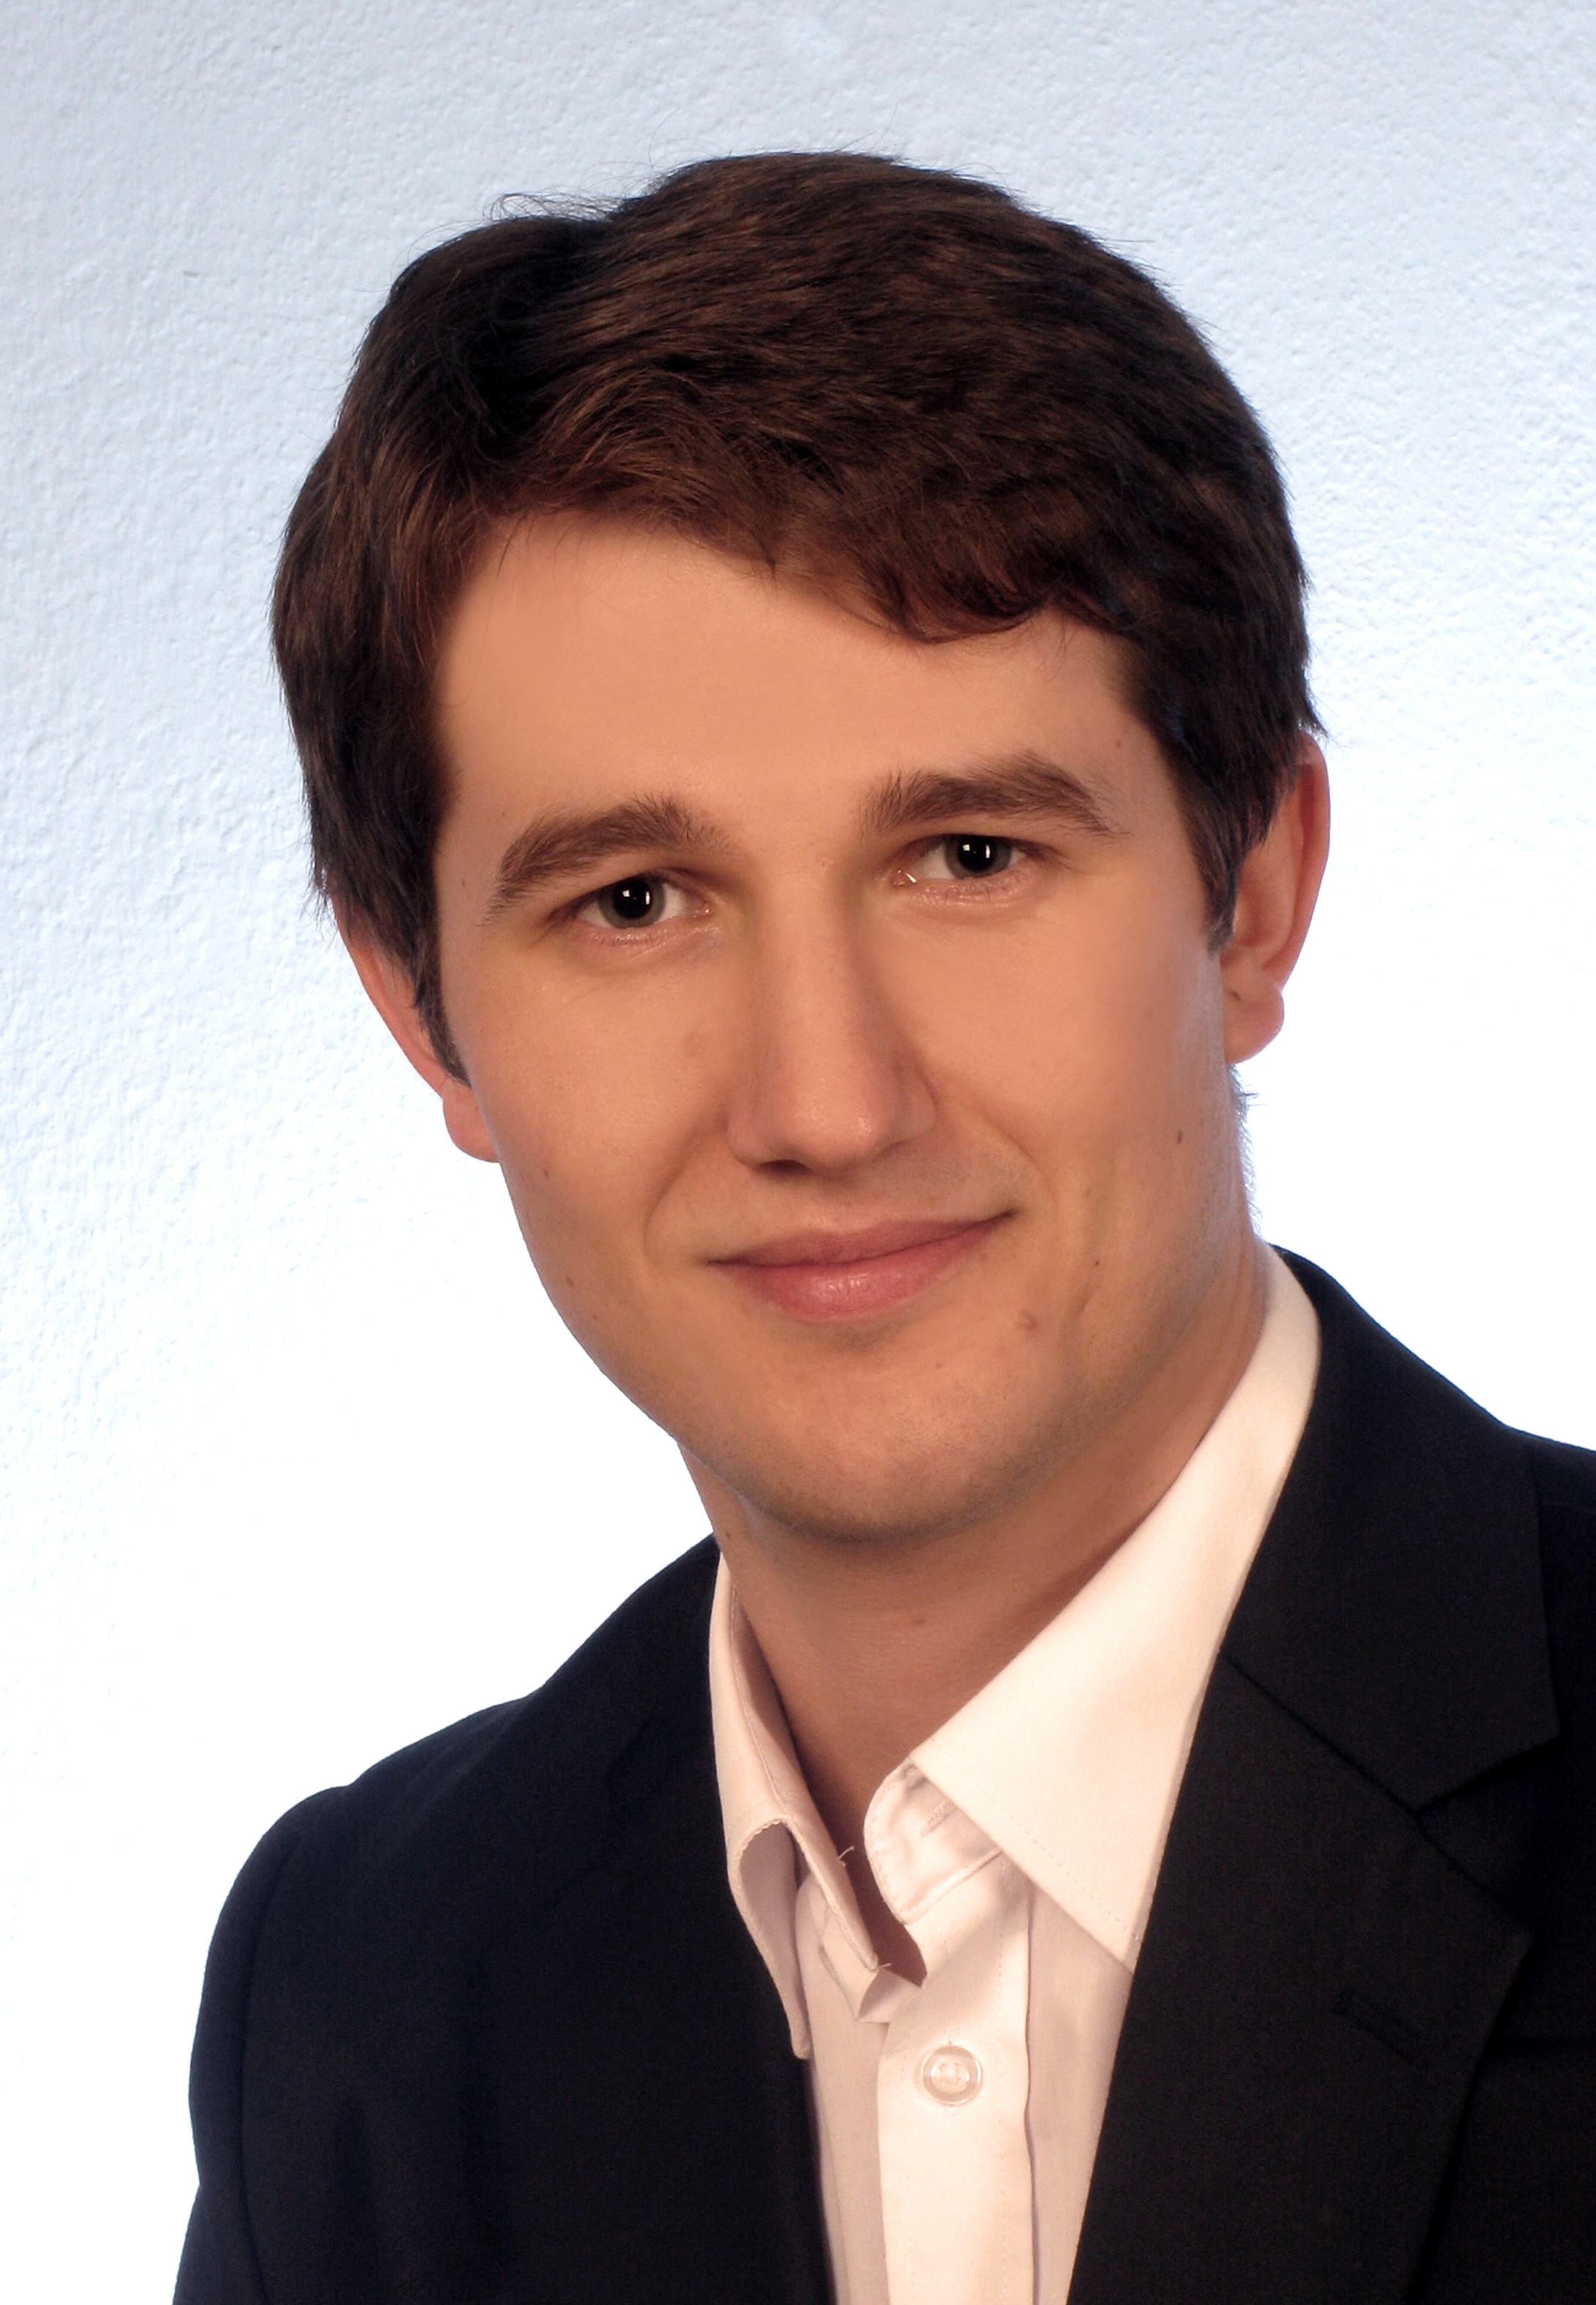
\includegraphics[height=6.5cm,width=4.5cm]{img/foto.jpg}
    \end{minipage}
    &
    \begin{minipage}{12cm}
    \begin{flushleft}
    \par\noindent\vspace{1\baselineskip}
    \begin{tabular}[h]{l l}
	{\normalsize\it Kierunek:} & {\normalsize Informatyka} \\ \\
    {\normalsize\it Specjalność:} & {\normalsize Inżynieria Systemów} \\ & {\normalsize Informatycznych}  \\ \\
    {\normalsize\it Data urodzenia:} & {\normalsize 12 grudnia 1991~r.} \\ \\
    {\normalsize\it Data rozpoczęcia studiów:} & {\normalsize 1 października 2010 r.} \\ \\
    \end{tabular}
    \par\noindent\vspace{1\baselineskip}
    \end{flushleft}
    \end{minipage}
    \end{tabular}
    \vspace*{1\baselineskip}
    \begin{center}
	{\large\bfseries Życiorys}\par\bigskip
    \end{center}

    \indent
    Urodziłem się 12 grudnia 1991 roku w Zamościu. W 2010 roku ukończyłem Społeczne Liceum Ogólnokształcące im. Unii Europejskiej w Zamościu. W październiku 2010 roku rozpocząłem studia na kierunku Informatyka na Wydziale Elektroniki i Technik Informacyjnych na Politechnice Warszawskiej. Od trzeciego roku studiów jestem na specjalizacji Inżynieria Systemów Informatycznych.
    \par
    \vspace{2\baselineskip}
    \hfill\parbox{15em}{{\small\dotfill}\\[-.3ex]
    \centerline{\footnotesize podpis studenta}}\par
    \vspace{1\baselineskip}
    \begin{center}
 	{\large\bfseries Egzamin dyplomowy} \par\bigskip\bigskip
    \end{center}
    \par\noindent\vspace{1.5\baselineskip}
    Złożył egzamin dyplomowy w dn. \dotfill
    \par\noindent\vspace{1.5\baselineskip}
    Z wynikiem \dotfill
    \par\noindent\vspace{1.5\baselineskip}
    Ogólny wynik studiów \dotfill
    \par\noindent\vspace{1.5\baselineskip}
    Dodatkowe wnioski i uwagi Komisji \dotfill
    \par\noindent\vspace{1.5\baselineskip}
    \dotfill

    % Streszczenie
    \newpage\thispagestyle{empty}
    \vspace*{2\baselineskip}
    \begin{center}
	{\large\bfseries Streszczenie}\par\bigskip
    \end{center}

    {\itshape
    Przedmiotem niniejszej pracy jest stworzenie systemu wspierającego ewidencje i tworzenie dokumentacji badań archeologicznych. Aplikacja ta została zaimplementowana z użyciem technologii zaproponowanej przez promotora - szkieletu aplikacji Vaadin - której zbadanie jest równoległym celem. Początek pracy poświęcony jest opisowi zakresu pracy. Następnie przedstawiony został opis systemu oraz wymagania mu stawiane. W dalszej części pracy są wymienione i opisane technologie, które zostały użyte do stworzenia systemu. Dalej przedstawiony jest opis implementacji z naciskiem na architekturę rozwiązania. W kolejnej części znajduje się przedstawienie produktów, które powstały przy okazji tworzenia systemu. Ostatnia część pracy zawiera podsumowanie oraz wnioski płynące z prac nad systemem.}
    \vspace*{1\baselineskip}

    \noindent{\bf Słowa kluczowe}: {\itshape Vaadin, Archeologia, Dokumentacja Archeologiczna}
    \par
    \vspace{4\baselineskip}
    \begin{center}
	{\large\bfseries Abstract}\par\bigskip
    \end{center}
    \noindent{\bf Title}: {\itshape 
	System to support the creation of archeological documentation created using Vaadin framework}\par
    \vspace*{1\baselineskip}
    {\itshape
    This thesis describes web application using three-tier architecture and Java programming language, which purpose was to support making documentation after archaeological research. The following chapters presentstages of application preparation. Whole graphic interface was made in framework Vaadin - which is described in detail in one of the chapters}
    \vspace*{1\baselineskip}

    \noindent{\bf Key words}: {\itshape Vaadin, Archeology, Archaeological Documentation}

\end{titlepage}

% ex: set tabstop=4 shiftwidth=4 softtabstop=4 noexpandtab fileformat=unix filetype=tex spelllang=pl,en spell:


\tableofcontents
% \addcontentsline{toc}{chapter}{{Przedmowa1}{vii}}{vii}

% \chapter*{Spis tablic, rysunków i~wydruków}
% \listoftables
% \listoffigures
% \lstlistoflistings

%\setlength{\baselineskip}{7mm}
\newpage
\pagenumbering{arabic}
\setcounter{page}{5}

\chapter{Wstęp}
W ostatnich latach, dzięki dynamicznemu rozwojowi informatyki, cyfryzacja jest widoczna w coraz to większej ilości gałęzi gospodarki. Nowoczesne przedsiębiorstwa zaczynają widzieć znaczne oszczędności dzięki wprowadzaniu do codziennej pracy systemów informatycznych. Szczególnym przykładem czynności, które mogłyby być a nawet powinny zostać zautomatyzowane są prace związane z wypełnianiem dokumentów, w których informacje wprowadzane przez pracownika są powielane w wielu miejscach. W bardziej popularnych branżach, rozwiązania usprawniające taką pracę są coraz częściej używane, jednak są także profile działalności w których informatyzacja byłaby pożądana, ale nie jest wprowadzana.

Jednym z przykładów działalności, gdzie systemy informatyczne usprawniły by pracę, jest firma prowadząca badania archeologiczne. Zwykłe prace na stanowisku archeologicznym sprowadzają się do fizycznego przebadania pewnego obszaru, a następnie stowrzenie dokumentacji podsumowującej wykonane prace oraz udokumentowującej obiekty archeologiczne oraz zabytki, z które zostały znalezionew trakcie badań.

W ostatnich latach, polski rynek badań archeologicznych staje się coraz większy, dzięki inwestycjom wziązanym z Unią Europejską. Badania archeologiczne prowadzone są na coraz większym obszarze, a co za tym idzie budżety firm archeologicznych są coraz większe. Niestety, wraz ze wzrostem skali badań, wzrasta też ilość dokumentacji, która jest produktem przeprowadzonych wykopalisk. Sytuacje komplikuje fakt, że w różnych województwach zdarza się, że są wymagane różne składniki dokumentacji. Dodatkowo, wraz ze wzrostem nakładów finansowych inwestowanych w badania archeologiczne zwiększyła się także liczba przedsiębiorst, które rywalizują ze sobą w przetargach. Większa konkurencja wymusza oczywiście spadek stawek za przeprowadzenie badań, dlatego firmy archeologiczne zmuszone są szczególnie do szukania oszczędności, których może dostarczyć cyfryzacja.

Na szczęście wraz z rozwojem informatyki idzie rozwój narzędzi do tworzenia systemów informatycznych. Szczególną gałęzią informatyki, która dzięki rozwojowi internetu zyskała na znaczeniu, są technologie tworzenia aplikacji internetowych. Jedną z technologii, która w niniejszej pracy została wybrana do stworzenia systemu, jest szkielet aplikacji Vaadin, który umożliwia szybkie tworzenie stron WWW. 
\newpage
\section{Cele i zakres pracy}
Głównym celem niniejszej pracy jest stworzenie systemu wspierającego działalność firmy "JN-Profil- badania archeologiczne i historyczne"  wspierającego ją w prowadzeniu badań archeologicznych. Drugim celem jest zapoznanie ze szkieletem aplikacji Vaadin, ułatwiającym tworzenie aplikacji internetowych. Dodatkowym, choć nieobowiązkowym celem jest storzenie komponentów graficznych ułatwiających wyświetlanie list obiektów i ich cech a także usprawniających tworzenie formularzy. 

System ewidencji badań archeologicznych, tworzony w ramach pracy, powinien umożliwiać wprowadzanie danych i generowanie dokumentacji archeologicznej w jak najbardziej przystępny i intuicyjny sposób. Aplikacja powinna także umożliwiać wprowadzanie danych dowolnym miejscu, ze względu na charakter działalności firmy archeologicznej - praca w różnych miejscach kraju.
\section{Układ pracy}
Rozdział 2. zawiera opis systemu ewidencji badań archeologicznych od strony inżynierii oprogramowania.

W rozdziale 3. znajduje się opis użytych technologii z uzasadnieniem wyboru.

Rozdział 4. zawiera opis technologiczny szkieletu aplikacji Vaadin, którego zbadanie jest celem niniejszej pracy.

Rozdział 5. opisuje proces tworzenia aplikacji oraz architekture rozwiązania.

W rozdziale 6. jest opisany proces testowania aplikacji.

Rozdział 7. opisuje produkty, które zostały dodatkowo wytworzone w trakcie budowy aplikacji.

Rozdział 8. zawiera wnioski wyciągnięte w procesie budowy systemu.

W rozdziale 9. znajduje się podsumowanie rezultatów pracy.

% ex: set tabstop=4 shiftwidth=4 softtabstop=4 noexpandtab fileformat=unix filetype=tex spelllang=pl,en spell:
\chapter{Analiza dziedziny problemu}
W dzisiejszych czasach, przed firmami archeologicznymi stoi nie małe wyzwanie, polegające na przeprowadzaniu badań archeologicznych na coraz większych powierzchniowo obszarach. Badanie archeologiczne przedinwestycyjne (w których specjalizuje się firma "JN-Profil" - docelowy użytkownik oprogramowania stworzonego w ramach niniejszej pracy) polegają na przeprowadzeniu badań terenowych oraz stworzeniu dokumentacji podsumowującej rezultaty tych badań.

Dokumentacja archeologiczna zawiera w sobie dużą liczbę dokumentów, z których conajmniej część opiera się na tych samych danych, których proces przetwarzania można, a nawet powinno sie zautomatyzować. Do tej pory, tworzenie dokumentacji sprowadzało się do mozolnego kopiowania danych z jednego miejsca do drugiego, jednak dzięki współcześnie dostępnym technologiom informatycznym istnieje możliwość zautomatyzowania i przyspieszenia tego procesu - co w szerszej perspektywie prowadzi do zmniejszenia kosztów przeprowadzania badań archeologicznych.

\section{Wymgagania biznesowe}
Przed systemem do prowadzenia ewidencji badań archeologicznych jest stawiany szereg wymagań, których spełnienie jest warunkiem poprawnego funkcjonowania oraz zadowolenia użytkowników. Część z nich jest wspólna dla wszystkich systemów informatycznych, natomiast reszta jest związana z charakterem pracy archeologa.

Aby system nadawał się do profesjonalnego użytku konieczne jest, aby efekty pracy były zapisane w pamięci trwałej. Konieczne jest także, aby możliwe było równoległe korzystanie wielu użytkowników, z dodatkowym zastrzerzeniem, że równoległe sesje użytkowników mogą pracować na tych samych danych i system powinien mimo to gwarantować spójność danych.

Specyficzną cechą pracy archeologa jest konieczność wyjazdów i prowadzenia badań archeologicznych w różnych miejscach. System wspierający prowadzenie ewidencji badań archeologicznych powinien umożliwiać tworzenie dokumentacji z różnych miejsc i urządzeń. 
\newpage
\section{Model dziedziny problemu}
W systemie wspierającym działalność firmy archeologicznej, powinno się wyróżnić 6 najważniejszych elementów:
\begin{itemize}
\item Zabytki Masowe\\
\item Zabytki Wydzielone\\
\item Obiekty Archeologiczne\\
\item Zdjęcia\\
\item Rysunki\\
\item Ary
\end{itemize}

Wszystkie powyższe obiekty są produktem przeprowadzanego badania archeologicznego, dlatego są bytami, które mają sens tylko w konkretnym kontekscie biznesowym (czyli opracowaniu). Wszystkie inne informacje wprowadzone do systemu są uniwersalne dla badań archeologicznych, dlatego są dostępne i edytowalne niezależnie od opracowania.
\newpage
\begin{figure} [H]
    \begin{center}
	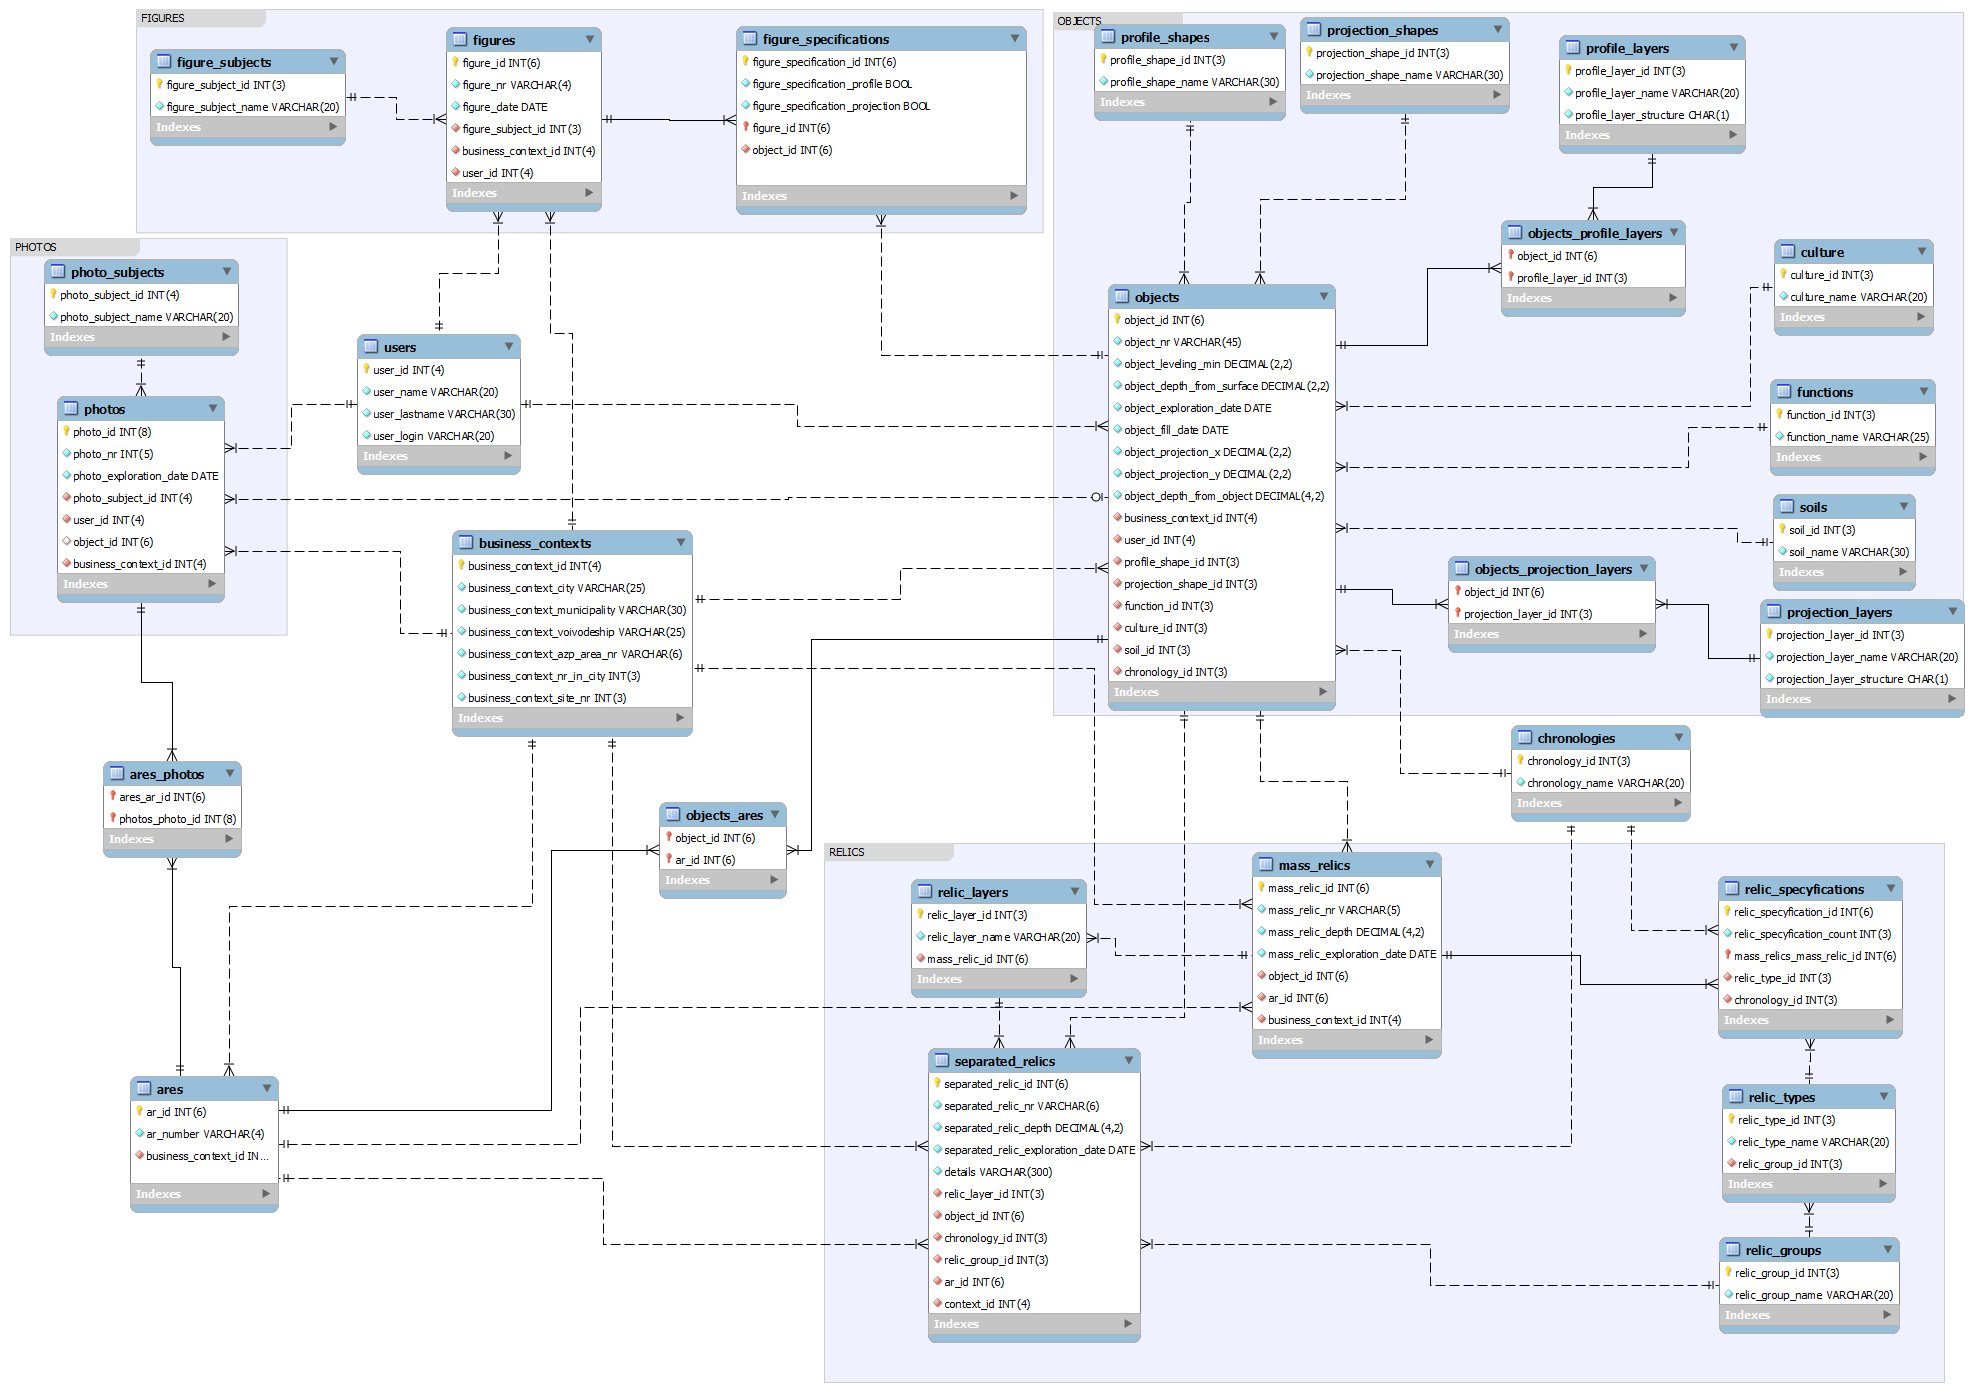
\includegraphics[angle=90, scale=.26]{img/db.png}
	\caption{Model dziedziny}
	\label{modelDziedziny}
    \end{center}
\end{figure}

\section{Model przypadków użycia}
Zadaniem systemu wspierającego tworzenie dokumentacji archeologicznej powinno być umożliwienie wprowadzenia danych w łatwy i przejrzysty sposób oraz szybkie generowanie raportów, będących składnikami dokumentacji archeologicznej.

\begin{figure} [H]
    \begin{center}
	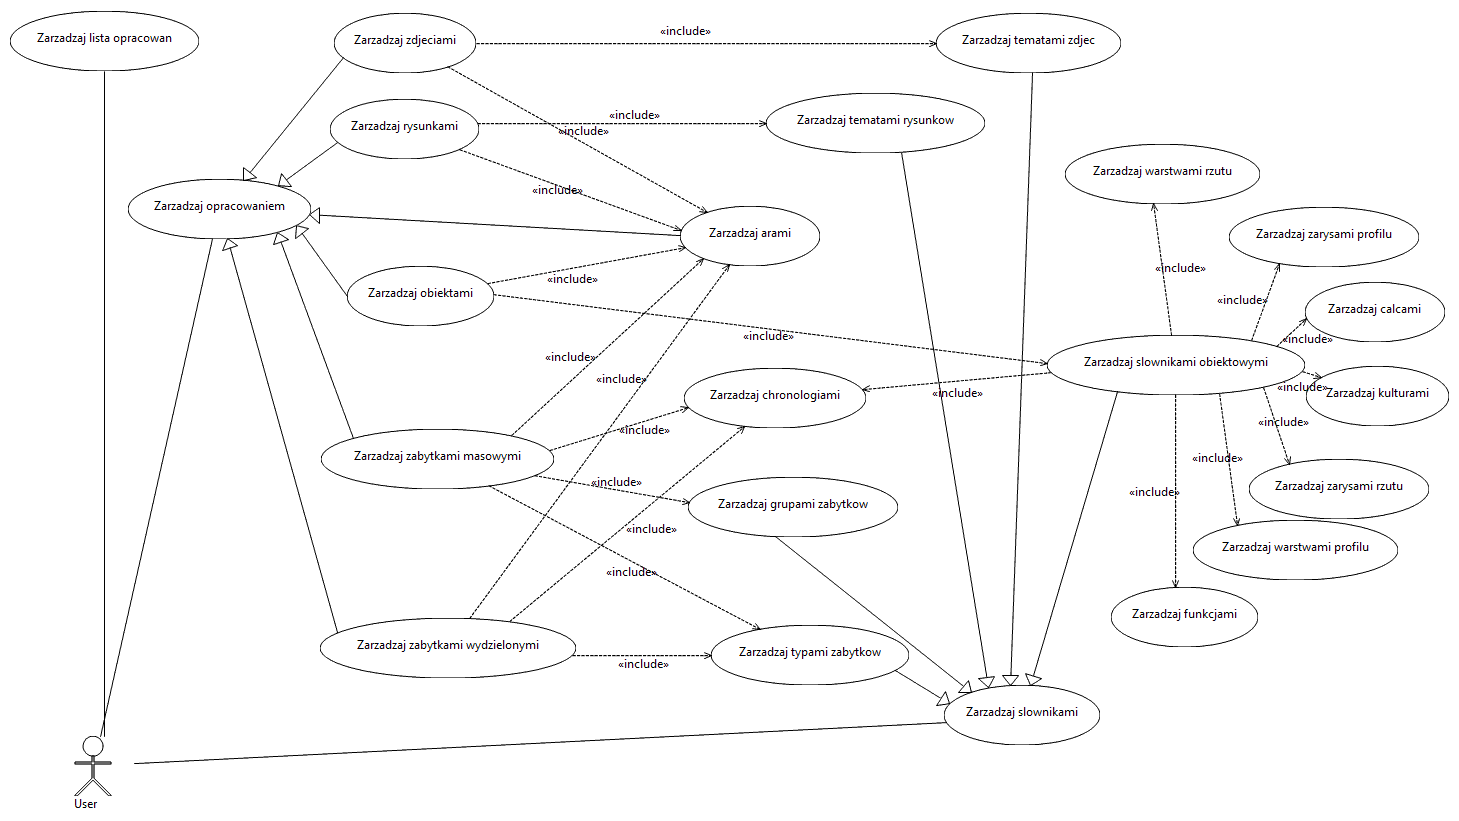
\includegraphics[angle=90, scale=.35]{img/useCasesData.png}
	\caption{Diagram przypadków użycia}
	\label{useCasesDiag}
    \end{center}
\end{figure}

Dodatkową cechą systemu będącego produktem niniejszej pracy jest to, że możliwa jest edycja słowników służących do wypełniania danych z poziomu okna edycji obiektu wypełnianego.
\newpage
\section{Struktura aplikacji}

Standardowy ekran aplikacji wygląda jak na poniższym rysunku.

\begin{figure} [H]
    \begin{center}
	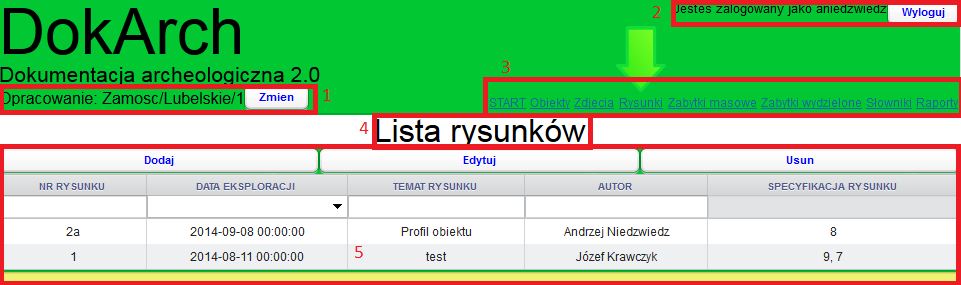
\includegraphics[scale=.6]{img/strona.png}
	\caption{Przykładowa podstrona systemu}
	\label{stronaPrzyklad}
    \end{center}
\end{figure}

Na załączonym obrazku widać, że strona aplikacji składa się z:
\begin{itemize}
\item górnej belki zawierającej w sobie informacje o bieżącym opracowaniu (1 na rysunku), informacje o zalogowanym użytkowniku (2) oraz menu (3)
\item belki tytułowej (4)
\item głównej treści strony (5) 
\end{itemize}

Powyższy rysunek demonstruje także przykładowy widok listujący wprowadzone dane (w tym przypadku rysunki). Dzięki addonowi FilterTable, możliwe jest filtrowanie widocznych elementów po ich zawartości w konkretnych polach. Standardowa funkcjonalność Vaadina pozwala także sortować wiersze wg wartości w kolumnie - w tym celu wystarczy kliknąć nagłówek kolumny.

\begin{figure} [H]
    \begin{center}
	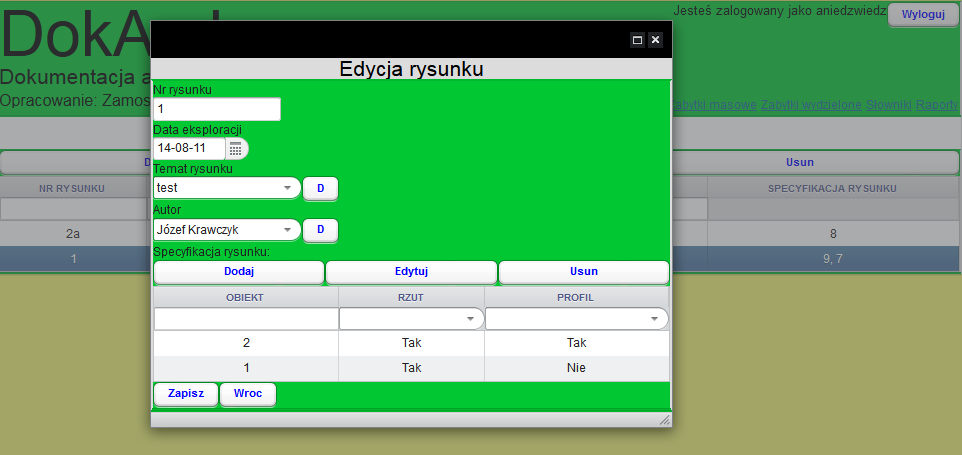
\includegraphics[scale=.6]{img/edycja.png}
	\caption{Przykładowa edycja obiektu dokumentacyjnego}
	\label{edycjaPrzyklad}
    \end{center}
\end{figure}

\newpage
Rysunek znajdujący się nad tym tekstem demonstruje ekran edycji wiersza (w tym przypadku wiersz odzwierciedla ewidencjonowany rysunek). 

\begin{figure} [H]
    \begin{center}
	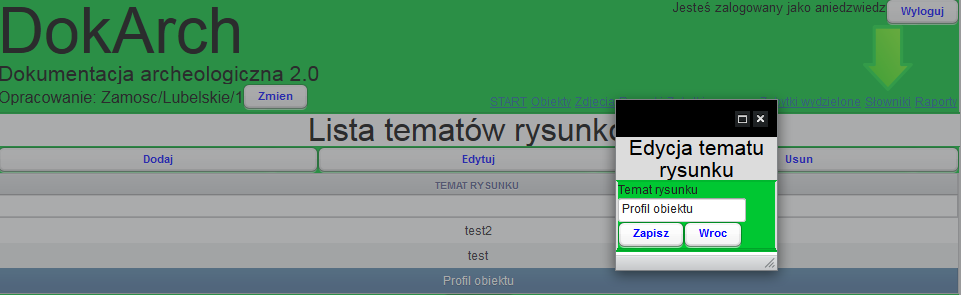
\includegraphics[scale=.6]{img/edycjaSlownika.png}
	\caption{Przykładowa edycja słownika}
	\label{edycjaSlownika}
    \end{center}
\end{figure}

Rysunek powyżej przedstawia standardowy sposób edycji słownika (wybranie w menu w górnej belce "Słowniki" a następnie wybranie słownika "Tematy rysunków"). Jest to jeden ze sposobów modyfikacji wartości słownika.

\begin{figure} [H]
    \begin{center}
	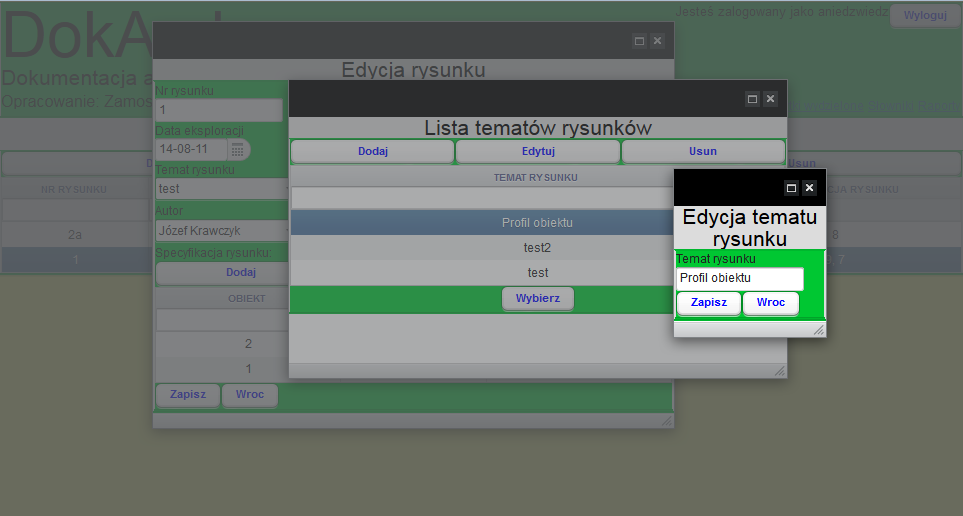
\includegraphics[scale=.6]{img/edycjaSlownikaWLocie.png}
	\caption{Przykładowa edycja słownika w trakcie edycji obiektu używającego go}
	\label{edycjaSlownikaWLocie}
    \end{center}
\end{figure}

Powyżej został przedstawiony ekran modyfikacji słownika w ``locie", czyli w trakcie edycji wiersza, który zawiera wartość ze słownika. Możliwe jest dynamiczne wprowadzanie wartości bez konieczności zamykania okna edycji.

% ex: set tabstop=4 shiftwidth=4 softtabstop=4 noexpandtab fileformat=unix filetype=tex spelllang=pl,en spell:
\chapter{Wykorzystane technologie}
Na rynku istnieje bardzo wiele szkieletów aplikacji i bibliotek usprawniających tworzenie aplikacji, w szczególności systemów wspomagających prace przedsiębiorstw, dlatego wybór technologii nie jest oczywisty. Jednym ze wspólnych kryteriów stawianych technologiom przy wyborze do tego projektu, był wymóg nieodpłatności za ich używanie, dlatego całe poniżej wymienione oprogramowanie jest bezpłatne.

(stos technologiczny - rysunek - TODO)

\section{MySQL}
Jednym z najważniejszych wymagań spoczywających na systemie informatycznym jest utrwalanie pracy użytkowników i radzenie sobie z ich równoległą pracą. We współczesnej informatyce, rola ta jest zazwyczaj oddelegowywana do specjalnie dedykowanych do tego celu programów nazwanych ogólnie bazami danych. Na rynku jest wiele systemów baz danych dlateg wybór nie jest oczywisty.

Podstawowy podział baz danych wg którego powinno rozpocząć się wybór oprogramowania jest na bazy relacyjne i tzw. NoSQL. Wydaje się jednak, że nierelacyjne bazy danych mają przewage w systemach, które są lub będą kiedyś duże, natomiast system ewidencji archeologicznej raczej nie ma szans być takim systemem. Z drugiej strony, relacyjne systemy baz danych były przez dłuższy czas uważane jako podstawowe, dlatego istnieje bardzo dużo informacji na ich temat w internecie, w przeciwieństwie to baz NoSQL, o których od niedawna dopiero zaczęło być głośniej.

Na rynku istnieje wiele relacyjnych systemów baz danych, jednak większość najpopularniejszych jest płatnych w rozwiązaniach komercyjnych. Wyjątkiem okazuje się MySQL, który pozwala korzystac w wersji bezpłatnej z bardzo szerokiej puli funkcjonalności, które w zupełności pokrywają potrzeby tworzonego przez autora systemu.
\newpage
\section{Hibernate}
Aby aplikacja mogła korzystać z bazy danych konieczne jest skomunikowanie ich ze sobą. Na rynku istnieje wiele narzędzi wspierających prace programisty, spośród których najpopularniejsze są JDBC i JPA. Ponieważ system będący wynikiem niniejszej pracy będzie operował na obiektach, warto byłoby użyć interfejsu programistycznego który umożliwia zapisywanie całych obiektów.

Java Persistence API to oficjalny standard mapowania relacyjno-obiektowego, który pozwala na utrwalanie obiektów w relacyjnej bazie danych. Jedną z implementacji będącą jednocześnie, najpopularniejszą jest Hibernate.

\begin{table}[H]
\caption{Liczba wątków z pytaniami związanymi z implementacją JPA}
\label{jpaImplementations}
\begin{center}
\begin{tabular}{|l|l|}
\multicolumn{1}{c}{Implementacja JPA} & \multicolumn{1}{c}{Ilość wątków} \\ \hline
Datanucleus & 682 \\ \hline
EclipseLink & 2745 \\ \hline
Hibernate & 37787 \\ \hline
TopLink & 240 \\ \hline
OpenJPA & 715 \\ \hline
\end{tabular} 
\end{center}
\end{table} 

Ze względu na niewielką styczność autora z dostępem do danych przez JPA, wybór padł na najbardziej popularny szkielet aplikacji - Hibernate.

\section{Spring Transaction Management}
Elementem nierozłącznym z relacyjną bazą danych jest transakcyjne przetwarzanie danych. Również w tym temacie istnieje wiele rozwiązań, dlatego nie ma potrzeby ręcznego implementowania fragmentów kodu odpowiedzialnego za zatwierdzanie bądź odrzucanie transakcji. W przypadku systemu tworzonego w ramach niniejszej pracy logika transakcji nie jest skomplikowana dlatego im prostsza implementacja tym bardziej preferowana.

Wybrane przez autora rozwiązanie, Spring Transaction Management, umożliwia wplatanie transakcji w istniejący kod w sposób przezroczysty. Po dodaniu do pliku konfiguracyjnego springa 4 linijek, programista jest w stanie tworzyć operacje na bazie danych w transakcjach po dopisaniu zaledwie jednej adnotacji definicją funkcji, w obrębie której odbywać się moją operacje na bazie danych.

\begin{lstlisting}
@Transactional
public void add(Figure f)
{
	getDaoObj().add(f);
}
\end{lstlisting}
\newpage
W jaki sposób jest otrzymywany powyższy efekt? Spring tworzy obiekt zdefiniowany przez programistę i opakowuje je w obiekt pośredniczący, który deleguje wszystkie operacje do obiektu właściwego, natomiast operacje oznaczone adnotacją @Transactional opakowuje w kod odpowiedzialny za transakcyjne przetwarzanie danych.

\section{Spring}
Jeszcze niedawno, dosyć dużym wyzwaniem było zarządzanie drzewem zależności obiektów wewnątrz aplikacji. W ostatnich latach, została jednak stworzona koncepcja wzorca projektowego polegającego na wstrzykiwaniu zależności bezpośrednio do obiektów ich używanych. Implementacja tego wzorca jest jeszcze łatwiejsza, dzięki powstaniu wielu bibliotek wspierających tego typu podejście.

Spring jako szkielet aplikacji zyskał na popularności przedewszystkim właśnie dzięki kontenerowi IoC (ang. Inversion-of-Control), który pozwala na łatwe tworzenie i zarządzanie zależności między obiektami. Wzorzec odwrócenia sterowania, będący pojeciem szerszym niż wstrzykiwanie zależności, pozwala skupić się na właściwej implementacji logiki a pozostawić zarządzanie zależnościami kontenerowi Springa, co znacznie ułatwia prace.

W dzisiejszych czasach, Spring jest jednym z najpopularniejszych szkieletów aplikacji, dlatego jednym z argumentów będących za jego użyciem jest bardzo duża ilość stron internetowych opisujących go oraz rozwiązujących potencjalne problemy w trakcie pracy z nim. 

\section{Logback + SLF4J}
Bardzo ważnym zagadnieniem, w kontekście tworzenia systemu informatycznego jest tworzenie logów aplikacji. Na rynku istnieje kilka rozwiązań dlatego wybór nie jest oczywisty. Aby uniezależnić się od wybranego rozwiązania, został oprócz implementacji biblioteki wspierającej logowanie, autor zdecydował się na przykrycie logowania warstwą abstrakcji umożliwiającą nieinwazyjne przełączenie się między realizacjami standardu logowania - SLF4J. 

Wybór w kwestii implementacji szkieletu aplikacji zapewniającego logowanie odbył się pomiędzy dwoma najpopularniejszymi - log4j oraz logback. Okazało się jednak, że logback jest kilkukrotnie szybszy niz log4j i zuzywa przy tym mniej pamięci (jak twierdzą autorzy tego pierwszego). Dodatkowo, przy zapoznawaniu sie z SLF4J okazało się, że logback wspiera natywnie ten standard, dlatego nie ma potrzeby używania modułu pośredniczącego miedzy slf4j i logbackiem, dzięki czemu można zyskać dodatkowo na szybkości działania aplikacji.

\newpage
\section{AspectJ}
Czy potrzebne? (todo)

\section{SpringSecurity}
Bardzo ważnym zagadnieniem, w implementacji systemów, szczególnie dostępnych w internecie, jest zapewnienie bezpieczeństwa. Aby dane gromadzone przez firme nie wpadły w niepowołane ręce, a szczególnie nie uległy zniszczeniu, konieczny jest szczelny sposób autoryzacji i autentykacji. Także i tej dziedzinie istnieje wiele rozwiązań wartych rozważenia.

Autor zdecydował się na SpringSecurity, będącym odrębnym bytem w stosunku do rdzenia Springa, jednak w prosty sposób się z nim integrującym. Implementacja ogranicza się do dopisania kilku linijek do pliku konfiguracyjnego springa, stworzenia strony odpowiadającej za zalogowanie i dodanie filtru do deskryptora wdrożenia (plik web.xml). Zaletą wybranego szkieletu aplikacji jest mnogość źródeł danych służących w procesie uwierzytelniania.

\section{LDAP - Apache Directory Server}
Innym zagadnieniem związanym z bezpieczeństwem jest miejsce przechowywania danych o użytkownikach, w szczególności ich loginów, haseł oraz uprawnień z nimi związanych. Standardowo, aplikacje przechowują takie informacje w bazie danych, jednak dla przedsiębiorstwa, którego liczba i skład pracowników zmienia się rzadko, mogą być także przechowywane w zewnętrznym serwerze takim jak LDAP.

Dodatkową korzyścią wynikającą z przechowywania danych użytkowników na serwerze LDAP jest możliwość posiadania centralnego punktu autoryzacji i autentykacji użytkowników w obrębie całej firmy. 

\section{Jasper reports (albo inny framework raportowy)}
(todo)

\newpage
\section{Tomcat}
Standardowy proces wdrażania aplikacji internetowych wymaga oprogramowania, które dostarcza środowisko uruchomieniowe. Powstało wiele tzw. kontenerów aplikacji webowych, które umożliwiają w prosty sposób uruchomić aplikacje napisane w języku Java jednocześnie udostępniając je w sieci. Część z nich, zwana serwerami aplikacji udostępnia dużo większy zakres możliwości i funkcjonalności, jednak nie były brane pod uwage, ze względu na stopień skomplikowania. 

Wybór autora padł na Apache Tomcat będącym jednym z najbardziej popularnych kontenerem aplikacji webowych. Dużą zaletą tego oprogramowania, oprócz łatwości i prostoty rozwiązania jest wsparcie środowiska programistycznego Eclipse, wybranego przez autora do stowrzenia implementacji systemu, do szybkiego wdrażania oprogramowania jeszcze w trakcie jego rozwijania. 
\section{Podsumowanie}
Wybrane przez autora technologie zostały dopasowane do potrzeb tworzonego systemu, dlatego przy tworzeniu każdego oprogramowania powinno się podchodzić indywidualnie do wyboru narzędzi wspierających budowe.

Należy także pamiętać, że technologie użyte przez autora do stworzenia systemu będącego tematem pracy, nie są uniwersalne - a wręcz przeciwnie - były aktualne i dosyć powrzechne w chwili pisania tej pracy. Bardzo prawdopodobne jest jednak, że za kilka lat zostaną uznane w środowisku informatycznym za przestarzałe, a w ich miejsce powstaną nowe, lepsze i/lub wydajniejsze.

% ex: set tabstop=4 shiftwidth=4 softtabstop=4 noexpandtab fileformat=unix filetype=tex spelllang=pl,en spell:
\chapter{Architektura rozwiązania}
\section{Model Widok Prezenter}
Aplikacje internetowe z reguły najlepiej wpisują się we wzorzec MVP (ang. Model-View-Presenter, Model-Widok-Prezenter), z którego autor postanowił skorzystać jako podstawe architektury systemu. Wzorzec ten polega na przekazaniu kontroli nad danymi prezentowanymi przez system do obiektu zwanego Prezenter. Mimo, że zdarzenia bezpośrednio pojawiają się w warstwie widoku, to natychmiast są one przekazywane do Prezentera, który w razie potrzeby odwołuje się do wartswy modelu i ewentualnie zmienia wygląd widoku prezentowanego użytkownikowi.

\begin{figure} [H]
    \begin{center}
	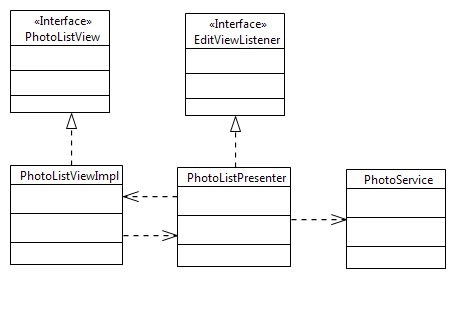
\includegraphics[scale=.8]{img/mvp.png}
	\caption{Przykład implementacji wzorca MVP}
	\label{mvp}
    \end{center}
\end{figure}

Powyższy rysunek przedstawia implementacje wzorca MVP w systemie wspierającym prowadzenie ewidencji badań archeologicznych. Na przykładzie widoku oraz prezentera listy zewidencjonowanych zdjęć pokazana jest współpraca komponentów.

\newpage
Aby maksymalnie rozluźnić zależności między obiektami zastosowane są interfejsy przez które komunikują się Widok z Prezenterem. Prezenter wystawia interfejs, który musi być implementowany przez widok, natomiast widok umożliwia jedynie rejestracje prezentera jako nasłuchiwacza zdarzeń. 

W chwili wystąpienia zdarzenia, np. chęci dodania nowego zdjęcia do listy, widok wywołuje odpowiadającą temu zdarzeniu metode na wszystkich obiektach zarejestrowanych jako nasłuchujące na obiekcie widoku. Prezenter otrzymuje w ten sposób notyfikacje, która może powodować np. komunikacje z baza danych przez obiekt PhotoService (np. dodanie do bazy danych nowego zdjęcia). Na zakończenie przetwarzania prezenter musi powiedzieć widokowi, że zmieniła się lista zdjęć. Aby utrzymać maksymalne rozluźnienie zależności, widok jest powiadamiany przez interfejs który implementuje.

\section{Podzial na pakiety}
Konsekwencją zastosowania wzorca MVP jest rozluźnienie zależności między obiektami, dzięki czemu w prosty sposób da się wyodrębnić luźno powiązane ze sobą moduły. W systemie zostały wyodrębnione 4 podstawowe pakiety:
\begin{itemize}
\item logic - pakiet zawierający definicje prezenterów oraz klas abstrakcyjnych z nimi powiązanych
\item gui - pakiet zawierający definicje widoków oraz klas abstrakcyjnych z nimi związanych
\item data - pakiet przechowujący kod procedur wykonujących operacje utrwalania danych
\item common - pakiet zawierający klasy wspólne dla klas z pakietów logic i gui
\end{itemize}

\begin{figure} [H]
    \begin{center}
	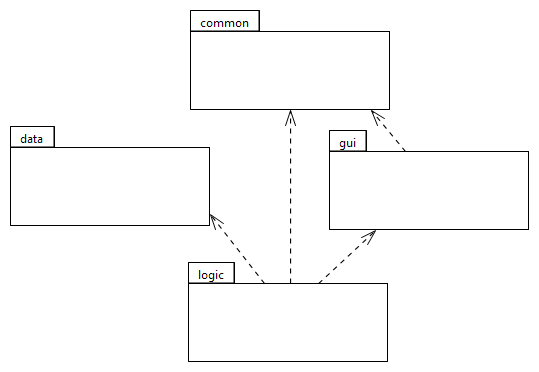
\includegraphics[scale=.6]{img/packageModel.png}
	\caption{Podział klas na pakiety}
	\label{packageModel}
    \end{center}
\end{figure}

\newpage
\section{Nawigacja między widokami}
Szkielet budowy aplikacji Vaadin sam w sobie posiada mechanizm przechodzenia między widokami, jest on jednak dosyć niewygodny w użyciu - istnieje konieczność rejestrowania widoków i ich adresów w momencie inicjalizacji obiektu UI. Na szczęście, dzięki wtyczce SpringVaadinIntegration możliwe jest przechodzenie między widokami jedynie po ich identyfikatorze w kontenerze Spring.

We wspomnianej przeze mnie wtyczce istnieje klasa implementująca powyższe zachowanie - DiscoveryNavigator. Wciąż jednak nie jest ona wystarczająca, jednak po przedefiniowaniu kilku metod okazuje się, że można dostosować ją do swoich potrzeb. 

Rozwiązanie wykorzystane w systemie będącym produktem niniejszej pracy wymaga zarejestrowania widoku w kontrolerze sesji, który na podstawie nazwy widoku nadaje powiązanie z nim odpowiedniemu prezenterowi. Prezenter z kolei, rejestruje się jako słuchacz zdarzeń widoku, którym steruje.

\section{Maksymalna abstrakcyjność}
System wspierający prowadzenie ewidencji dokumentacji archeologicznej musi umożliwiac wprowadzanie wielu rodzajów danych. Wiąże się to z dużą ilością klas z kategorii widoków i prezenterów. Szczególnie w przypadku słowników, istnieje wielka szansa na konieczność wielokrotnego powtarzania tych samych fragmentów kodu, stąd ambicją autora było stworzenie szkieletu aplikacji skracającego czas tworzenia komponentów odpowiedzialnych za wprowadzanie danych do systemu do minimum.

Szkielet aplikacji, o którym była mowa w poprzednim akapicie wymaga dwóch osobnych struktur hierarchii obiektów, jednek dla widoków i jednej dla prezenterów. Konieczne jest także, aby te struktury wzajemniej były od siebie zależne, zgodnie ze wzorcem MVP opisanym w pierwszej części tego rozdziału.

Poniżej zostało zaprezentowane drzewo dziedziczenia widoków, powstałe w wyniku projektu aplikacji, który następnie w trakcie implementacji został delikatnie zmodyfikowany. 

\begin{figure} [H]
    \begin{center}
	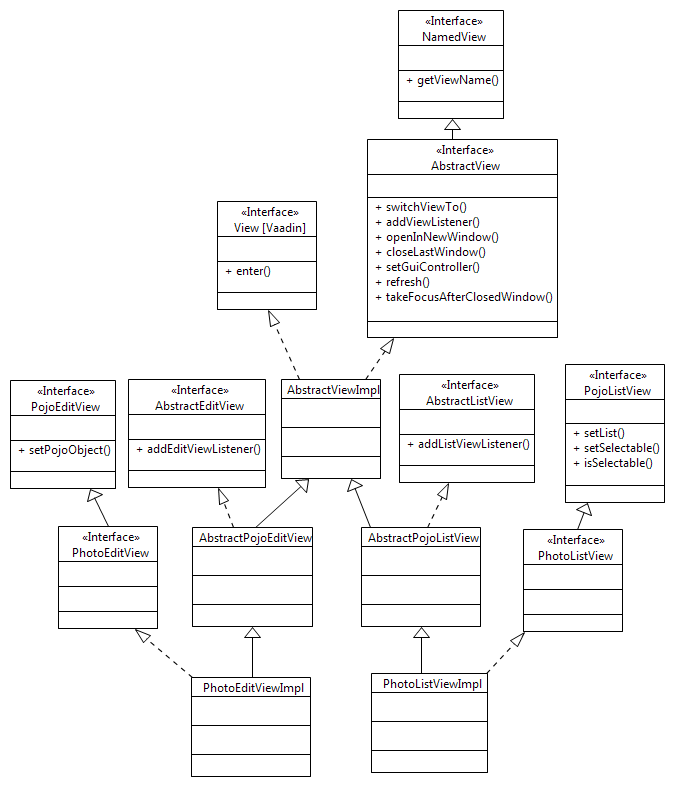
\includegraphics[scale=.55]{img/viewHierarchy.png}
	\caption{Hierarcha widoków}
	\label{viewHierarchy}
    \end{center}
\end{figure}

Na samej górze hierarchii znajduje się interfejs wymuszony przez technologie Vaadin (View), która jest konieczna do wyświetlenia różnych widoków w obrębie jednego obiektu UI. Drugim korzeniem hierarchii jest interfejs NamedView, który pozwala nadawać nazwy widokom, co z kolei utożsamiane jest z nazwą odpowiadającego komponentu Springa (ang. bean) a także przydzielanego fragmentu URI, doczepianego do adresu i pozwalającego przeglądarce zapamiętywać historie nawigacji po stronie.

Całe drzewo dziedziczenia wyraźnie podzielone jest na dwie części - obiekty widoków listy i widoków okna edycji wiersza. Jest to spowodowane oczywiście różnymi zadaniami stawianymi obiektom implementującym powyższe funkcje.

\newpage
Rdzeń implementacji znajduje się w klasach AbstractViewImpl oraz AbstractPojoEditView i AbstractPojoListView. AbstractViewImpl jest klasą z której bezpośrednio dziedziczą wszystkie "standardowe" widoki prezentujące zwykłą treść, np. lista słowników czy strona startowa. AbstractPojoEditView jest z kolei klasą po której bezpośrednio dziedziczą wszystkie implementacje widoków okien edycji użyte w systemie. Implementuje ona wygląd okna edycji (za pomocą klasy DefaultForm, opisanej w rozdziale 7., która dynamicznie generuje wygląd formularza na podstawie adnotacji zawartych w klasie obiektu edytowanego) oraz całą obsługe przekazywania zdarzeń, które zostały wygenerowane przez użytkownika, czyli wywołuje metody na obiektach nasłuchiwaczy (czyli prezenterów).

Warto także dodać, że hierarchia jest skonstruowana w ten sposób, aby uniezależnić maksymalnie reszte klas wchodzących w skład pakietu obsługującego cały interfejs graficzny użytkownika, od technologii prezentacji, którą w tym przypadku jest Vaadin.

\newpage
\begin{figure} [H]
    \begin{center}
	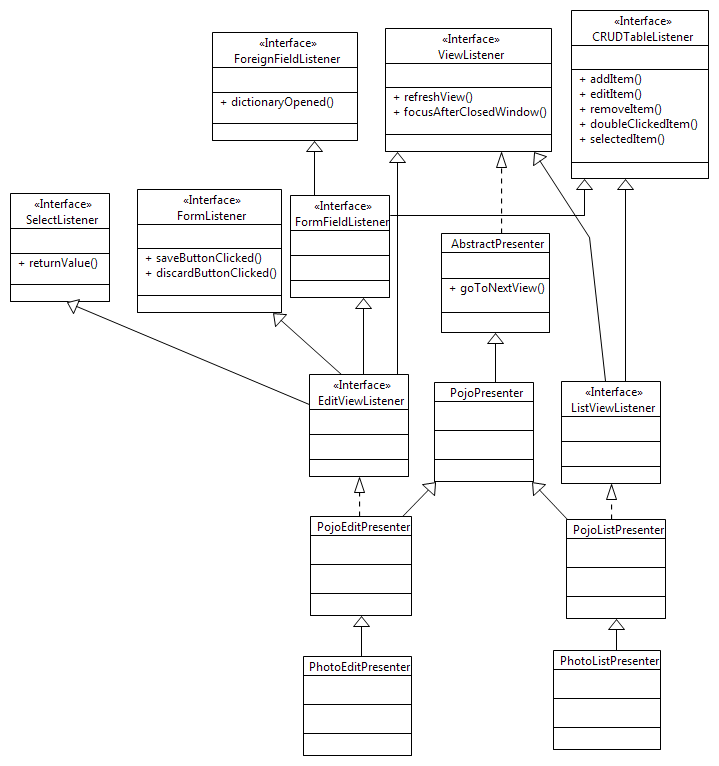
\includegraphics[scale=.6]{img/presenterDiagram.png}
	\caption{Hierarchia prezenterów}
	\label{presenterHierarchy}
    \end{center}
\end{figure}

Powyżej została przedstawiona hierarchia prezenterów w szkielecie aplikacji stworzonym przez autora w trakcie tworzenia systemu ewidencji badań archeologicznych. Na samym początku warto zaznaczyć, że hierarchia ta jest tak rozbudowana, ze względu na dopasowanie do komponentów stworzonych w trakcie pracy nad systemem - ForeignField oraz CRUDTable, które są opisane w rodziale 7.

Dodatkowo, wszystkie widoki użyte w systemie muszą implementować interfejs ViewListener, który pozwala reagować na ogólne zachowania widoków, a mówiąc ściślej, pozwala wykonywać akcje przy okazji przejścia z jednego widoku do drugiego - np. odświerzenie zawartości. 

\newpage
Każdy prezenter w systemie powinien także dziedziczyć po klasie AbstractPresenter, pozwala implementuje elementy związane z nawigacją (pamięta który prezenter jest jego "rodzicem" - czyli jest prezenterem widoku który wywołał ten widok oraz implementuje przejście do następnego widoku).

Tak jak w przypadku hierarchii widoków, tak w przypadku prezenterów konieczne jest rozdzielenie na dwie główne gałęzie - prezenterów okna edycji oraz prezenterów listy obiektów. Gałęzie te mają swoją implementacje kolejno w klasach: PojoEditPresenter i PojoListPresenter. Głównym zadaniem wymienionych klas jest implementacja reakcji na działania użytkownika, które zostały przekazane dalej przez widok poprzez interfejs nasłuchiwacza (zaimplementowany w tych właśnie klasach). Na samym dole hierarchii znajdują się klasy konkretne, odpowiadające prezenterom obiektów dziedziny problemu. Poniżej przykład implementacji prezentera okna edycji:
\begin{lstlisting}
@Component
@Scope("session")
public class FigureSubjectEditPresenter 
			extends PojoEditPresenter<FigureSubject>
{
	public interface FigureSubjectEditView 
			extends PojoEditView<FigureSubject>
	{
	}

	@Autowired
	public FigureSubjectEditPresenter(
			FigureSubjectEditView pojoEditView, 
			AbstractServiceInterface<FigureSubject> pojoServ)
	{
		setView(pojoEditView);
		setPojoService(pojoServ);
	}
}
\end{lstlisting}

Jak widać, powyższy kod implementuje się bardzo szybko. Dodatkową prostote autor osiągnął dzięki zastosowaniu kontenera IoC Springa, który wstrzykuje zależności bezpośrednio do konstruktora, za pomocą adnotacji @Autowired. Warto zwrócić uwagę, że każda klasa konkretna definiuje swój odrębny interfejs widoku, który jednak standardowo posiada takie same metody jak wszystkie inne w tej grupie widoków (okno edycji).

\newpage
Klasa przedstawiona na listingu jest prezenterem okna edycji obiektu, który nie posiada ani kolekcji obiektów podrzędnych (związek Jeden-Do-Wielu oraz Wiele-Do-Wielu) ani obiektów pochodzących ze słownika. Jeżeli by tak było, konieczne byłoby zaimplementowanie dodatkowych metod:
\begin{itemize}
\item getDataProvider() - metoda zwracająca obiekt implementujący interfejs DataProvider, używany w kontekście słowników do wypełniania wartości
\item getDictionaryPresenter() - metoda zwracająca, na podstawie argumentu, prezenter używany przez widok powiązany z danym słownikiem
\item getActiveFieldPresenter() - metoda zwracająca, na podstawie argumentu, prezenter używany przez widok powiązany z jednym z obiektów kolekcji (powinien to być Prezenter Listy w przypadku związku Wiele-Do-Wielu oraz prezenter okna edycji obiektu podrzędnego w przypadku związku Jeden-Do-Wielu, np. specyfikacja rysunku).
\item fillValueInOneToManyRel() - metoda, która wzbogaca obiekt zwrócony z potomnego prezentera, o referencje do obiektu prezentowanego
\end{itemize}

Kod prezentera listy obiektów jest niewiele bardziej skomplikowany:
\begin{lstlisting}
@Component
@Scope("session")
public class FigureSubjectListPresenter 
			extends PojoListPresenter<FigureSubject>
{
	public interface FigureSubjectListView 
				extends PojoListView<FigureSubject>
	{
	}

	@Autowired
	public FigureSubjectListPresenter(
			AbstractServiceInterface<FigureSubject> pojoServ, 
			FigureSubjectListView pojoListView,
			FigureSubjectEditPresenter photoSubjectEditPres)
	{
		super(FigureSubject.class);
		setPojoService(pojoServ);
		setPojoListView(pojoListView);
		setPojoEditPresenter(photoSubjectEditPres);
	}
\end{lstlisting}
\newpage
\begin{lstlisting}
	@Override
	protected Criterion getCriterion()
	{
		return null;
	}

	@Override
	protected FigureSubject getEmptyObject()
	{
		return new FigureSubject();
	}
}
\end{lstlisting}
Ten prezenter także zawiera definicje interfejsu widoku, z którym się komunikuje oraz także w tym przypadku użyty został kontener Springa wstrzykujący zależności bezpośrednio do konstruktora.

Dodatkowo pojawiły się dwie proste metody:
\begin{itemize}
\item getCriterion() - zwracająca kryterium służące do wyboru listy elementów prezentowanych
\item getEmptyObject() - tworzący nowy obiekt, zgodnie ze wzorcem fabryka
\end{itemize}

Jak widać na przykładach powyżej, cała implementacja reakcji prezenterów na zdarzenia przychodzące z interfejsu graficznego użytkownika jest zaimplementowana w klasach abstrakcyjnych, natomiast w klasach konretnych zostało jedynie ustawienie wartości konkretnych pól a także zaimplementowanie odpowiednich abstrakcyjnych metod, które są użyte w klasach abstrakcyjnych.
% ex: set tabstop=4 shiftwidth=4 softtabstop=4 noexpandtab fileformat=unix filetype=tex spelllang=pl,en spell:
\chapter{Prezentacja aplikacji}
W niniejszym rozdziale zostanie zaprezentowany od strony użytkowej system, który powstał w ramach niniejszej pracy.

W momencie rozpoczęcia nowej sesji, użytkownikowi pokazuje się ekran logowania:

\begin{figure} [H]
    \begin{center}
	
\includegraphics[scale=.6]{img/ekranLogowania.png}
	\caption{Ekran logowania}
	\label{stronaPrzyklad}
    \end{center}
\end{figure}

Następnie, bo zalogowaniu, użytkownikowi jest wyświetlane okno wyboru opracowania (na poniższym rysunku). Ekran ten jest widoczny na samym początku sesji, ale może też być wyświetlony w dowolnym momencie użytkowania systemu, poprzez kliknięcie przycisku "Zmień" w sekcji opracowanie, w górnej belce strony. Z poziomu wyświetlonego ekranu użytkownik może dodawać, edytować bądź usuwać (tylko te, dla których nie zostały dodane żadne dane) opracowania. W ten sposób jest spełniony przypadek użycia UC1. - Zarządzaj listą opracowań.
\begin{figure} [H]
    \begin{center}
	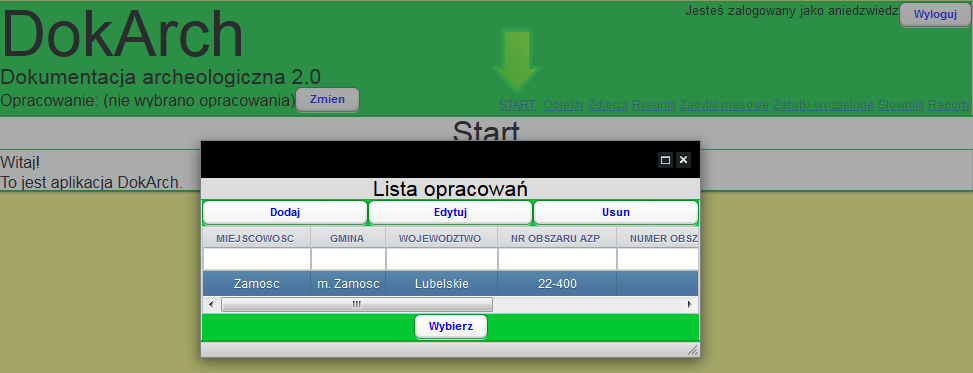
\includegraphics[scale=.6]{img/ekranStartowy.png}
	\caption{Ekran logowania}
	\label{stronaPrzyklad}
    \end{center}
\end{figure}
\newpage
Standardowy ekran aplikacji wyświetlający liste elementów wygląda jak na poniższym rysunku.

\begin{figure} [H]
    \begin{center}
	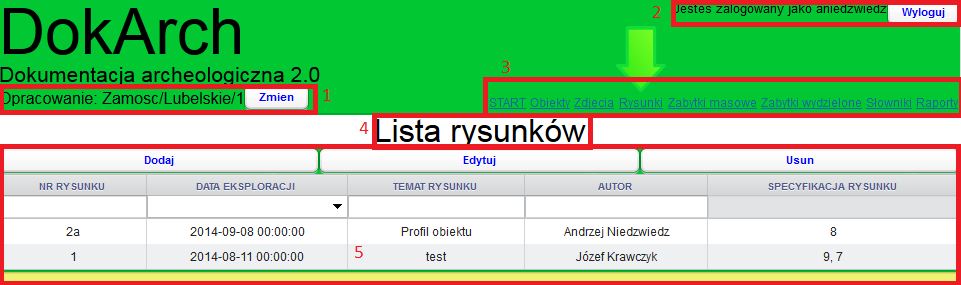
\includegraphics[scale=.6]{img/strona.png}
	\caption{Przykładowa podstrona systemu}
	\label{stronaPrzyklad}
    \end{center}
\end{figure}

Na załączonym obrazku widać, że strona aplikacji składa się z:
\begin{itemize}
\item górnej belki zawierającej w sobie informacje o bieżącym opracowaniu (1 na rysunku), informacje o zalogowanym użytkowniku (2) oraz menu (3)
\item belki tytułowej (4)
\item głównej treści strony (5) 
\end{itemize}

Powyższy rysunek demonstruje także przykładowy widok listujący wprowadzone dane (w tym przypadku rysunki). Dzięki addonowi FilterTable, możliwe jest filtrowanie widocznych elementów po ich zawartości w konkretnych polach. Standardowa funkcjonalność Vaadina pozwala także sortować wiersze wg wartości w kolumnie - w tym celu wystarczy kliknąć nagłówek kolumny.

\begin{figure} [H]
    \begin{center}
	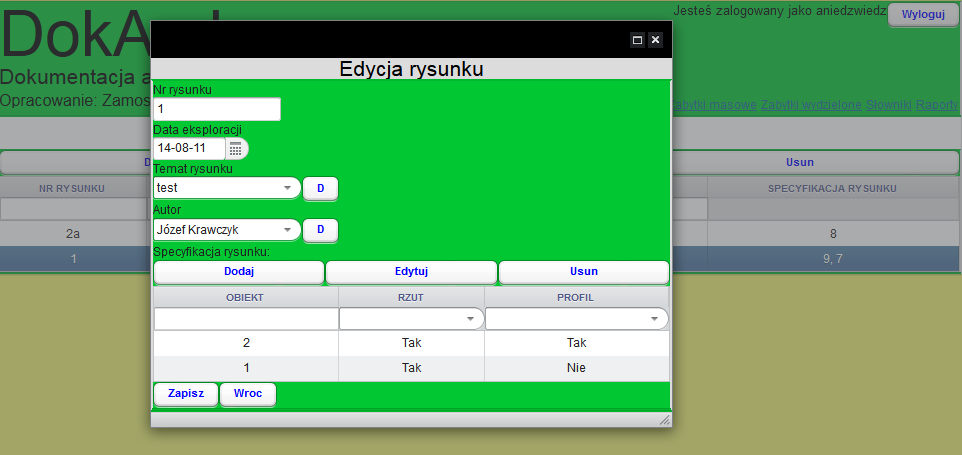
\includegraphics[scale=.6]{img/edycja.png}
	\caption{Przykładowa edycja obiektu dokumentacyjnego}
	\label{edycjaPrzyklad}
    \end{center}
\end{figure}

\newpage
Rysunek znajdujący się nad tym tekstem demonstruje ekran edycji wiersza (w tym przypadku wiersz odzwierciedla ewidencjonowany rysunek). Ten sam ekran (tylko z niewypelnionymi wartościami) jest wyświetlany użytkownikowi po otrzymaniu informacji o wciśnięciu przez użytkownika przycisku dodaj. Lista wysunków wraz z oknem edycji rysunków wypełniają przypadek użycia "UC5. Zarządzaj rysunkami".

\begin{figure} [H]
    \begin{center}
	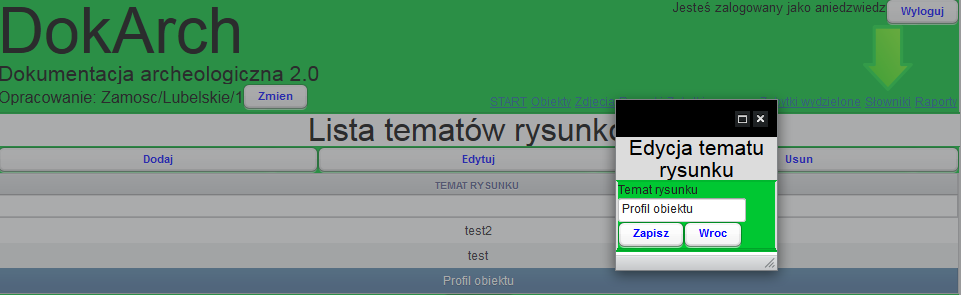
\includegraphics[scale=.6]{img/edycjaSlownika.png}
	\caption{Przykładowa edycja słownika}
	\label{edycjaSlownika}
    \end{center}
\end{figure}

Rysunek powyżej przedstawia standardowy sposób edycji słownika (wybranie w menu w górnej belce "Słowniki" a następnie wybranie słownika "Tematy rysunków"). Jest to jeden ze sposobów modyfikacji wartości słownika.

\begin{figure} [H]
    \begin{center}
	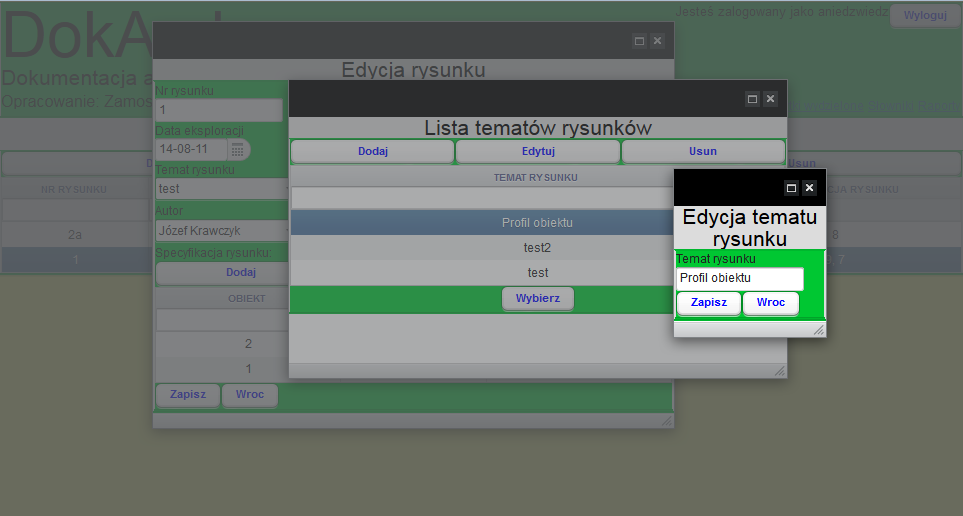
\includegraphics[scale=.6]{img/edycjaSlownikaWLocie.png}
	\caption{Przykładowa edycja słownika w trakcie edycji obiektu go używającego}
	\label{edycjaSlownikaWLocie}
    \end{center}
\end{figure}

\newpage
Powyżej został przedstawiony ekran modyfikacji słownika w ``locie", czyli w trakcie edycji wiersza, który zawiera wartość ze słownika. Możliwe jest dynamiczne wprowadzanie wartości bez konieczności zamykania okna edycji.

Wyświetlenie listy wartości oraz ich modyfikacja może nastąpić na dwa sposoby. Pierwszy sposób to wybranie przycisku D przy polu słownikowym. Wtedy otwiera się okno z tabelką widoczne poniżej:

\begin{figure} [H]
    \begin{center}
	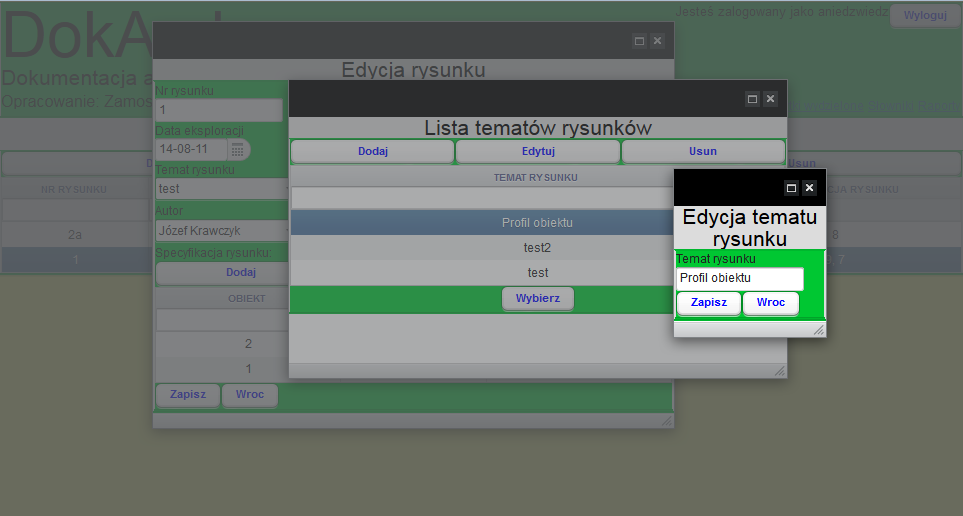
\includegraphics[scale=.6]{img/edycjaSlownikaWLocie.png}
	\caption{Lista tematów rysunków zmieniana w ``locie''}
	\label{edycjaListySlownikaWLocie}
    \end{center}
\end{figure}

Drugim sposobem jest kliknięcie w link w menu strony w nazwie "Słowniki". Link ten przeniesie użytkownika do strony widocznej poniżej:

\begin{figure} [H]
    \begin{center}
	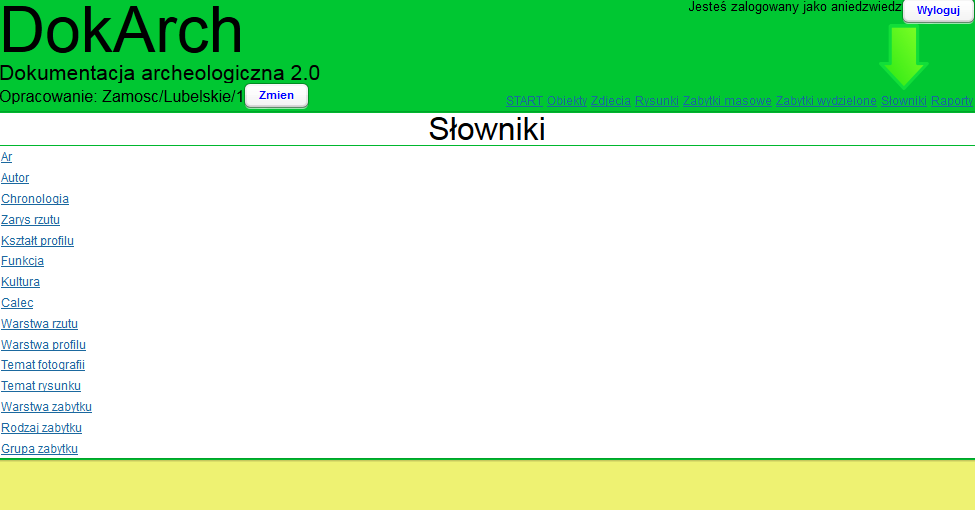
\includegraphics[scale=.6]{img/listaSlownikow.png}
	\caption{Lista słowników}
	\label{listaSlownikow}
    \end{center}
\end{figure}
\newpage
Następnie użytkownik wybiera interesujący go słownik i klika w link prowadzący do niego. Przykładowy słownik po wciśnięciu linka:

\begin{figure} [H]
    \begin{center}
	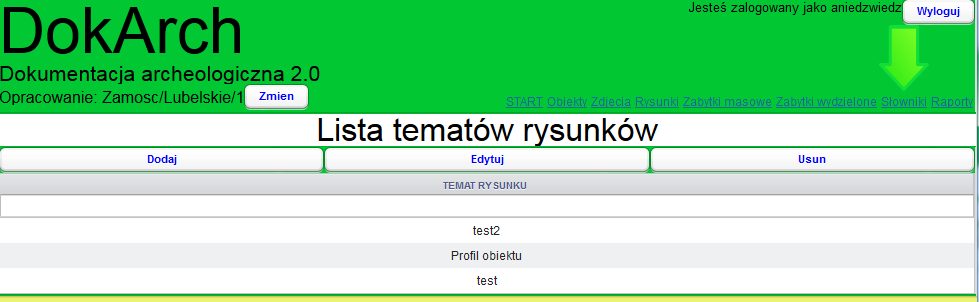
\includegraphics[scale=.6]{img/listaTematowRysunkow.png}
	\caption{Lista tematów rysunków}
	\label{listaTematowRysunkow}
    \end{center}
\end{figure}

W ten sposób pokazano, że system ma zaimplementowany przypadek użycia UC9. Zarządzaj tematami rysunków.

System potrafi także generować raporty. Aby tego dokonać wystarczy kliknąc link w menu "Raporty", i wybrać interesujący raport z listy:

\begin{figure} [H]
    \begin{center}
	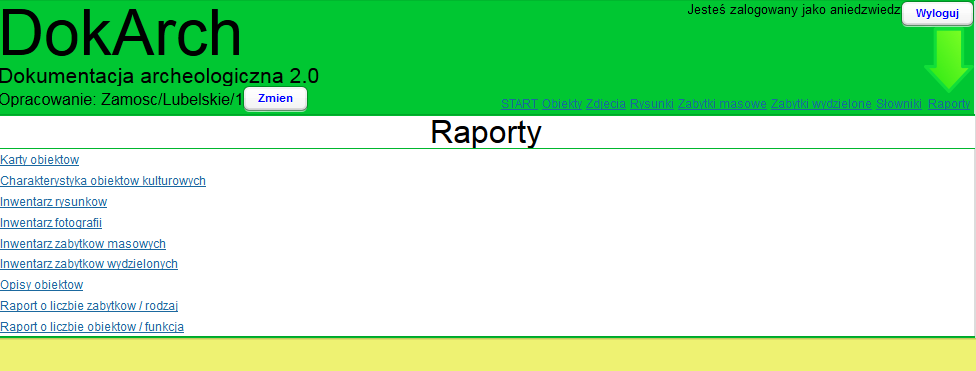
\includegraphics[scale=.6]{img/ekranRaportow.png}
	\caption{Ekran raportów}
	\label{listaRaportow}
    \end{center}
\end{figure}
\newpage
Przykładowy raport wygenerowany przez system:

\begin{figure} [H]
    \begin{center}
	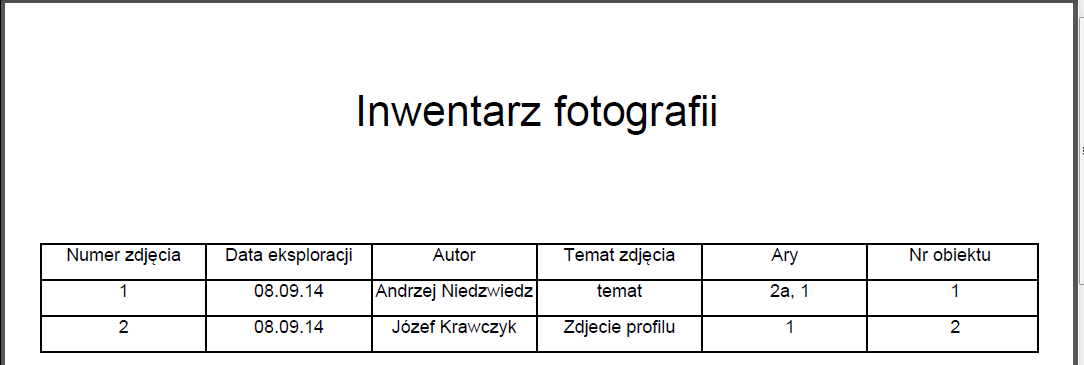
\includegraphics[scale=.6]{img/przykladowyRaport.png}
	\caption{Przykładowy raport}
	\label{przykladowyRaport}
    \end{center}
\end{figure}

% ex: set tabstop=4 shiftwidth=4 softtabstop=4 noexpandtab fileformat=unix filetype=tex spelllang=pl,en spell:
\chapter{Dodatkowe produkty pracy}
W trakcie tworzenia niniejszej pracy powstało także kilka produktów ubocznych, które zdaniem autora mają szanse zostać popularnymi wtyczkami do szkieletu aplikacji Vaadin oraz o których warto wspomnieć. Każda z tych wtyczek używa adnotacji zaszytych bezpośrednio w klasie obiektu na których operują.

\section{Standardowa klasa POJO}
Poniżej została przedstawiona uproszczona standardowa klasa zawierająca konfiguracje z użyciem adnotacji używana przez wymienione w tym rozdziale komponenty.
\begin{lstlisting}
@Entity
@Table(name = "figure_specifications")
@ForeignFieldLabel(pattern = "id")
public class FigureSpecification
{
	@Id
	@GeneratedValue
	@Column(name = "figure_specification_id")
	private Long id;

	@Column(name = "figure_specification_profile")
	@ColumnHeader(value = "Profil", order = 3)
	@EditField(label = "Profil", order = 3)
	@NotNull
	private Boolean profile = false;

	@Column(name = "figure_specification_projection")
	@ColumnHeader(value = "Rzut", order = 2)
	@EditField(label = "Rzut", order = 2)
	@NotNull
	private Boolean projection = false;
\end{lstlisting}
\newpage
\begin{lstlisting}
	@JoinColumn(name = "figure_id")
	@NotNull(message = "Rysunek nie moze byc pusty")
	@ManyToOne(optional = false)
	private Figure figure;

	@JoinColumn(name = "object_id")
	@ColumnHeader(value = "Obiekt", order = 1)
	@EditField(label = "Obiekt", order = 1)
	@NotNull(message = "Obiekt nie moze byc pusty")
	@ManyToOne(optional = false)
	private ArchObject archObject;
	...
	(gettery i settery)
}
\end{lstlisting}
Jak widać, w powyższej klasie zostały użyte trzy typy adnotacji:
\begin{itemize}
\item javax.persistence - odpowiedzialne za mapowanie relacyjno-obiektowe wewnątrz systemu
\item javax.validation - odpowiedzialne za walidacje wprowadzonych wartości
\item dedykowane dla stworzonych komponentów
\end{itemize}
Jak dalej zostanie opisane w tym rozdziale, każdy z wyżej wymienionych rodzajów jest wykorzystywany przez niżej opisane komponenty.

Warto zwrócić także uwagę na adnotacje @ForeignFieldLabel, zawierającą definicje sposobu wyświetlania obiektu POJO w poniższych komponentach. Składnia wyrażenia zawartego w adnotacji pozwala wyświetlać zarówno pojedyńcze pole (wartość "nazwa\_pola" lub "\$nazwa\_pola\$") lub kombinacje jednego bądź większej ilości pól ze statycznym ciągiem znaków (np. "Pan: \$imie\$ \$nazwisko\$", nazwy zmiennych zawierają sie między znakami "\$"). Jedynym warunkiem poprawnego wyświetlenia napisu odpowiadającego wartościom obiektu jest konieczność implementowania przez użyte pola metody toString().

\section{CRUDTable}
CRUDTable to komponent, który wyświetla liste obiektów wykorzystując wtyczkę FilterTable opartą na komponencie CustomTable wzbogacona o standardowe przyciski generujące akcje związane z przetwarzaniem danych tabelarycznych, tzn. dodawania, edytowania i usuwania wierszy. Dodatkowo, zaimplementowana jest funkcjonalność z użyciem wtyczki ContextMenu, która zawiera domyślnie także akcje związane z przetwarzaniem zbioru danych.

\begin{figure} [H]
    \begin{center}
	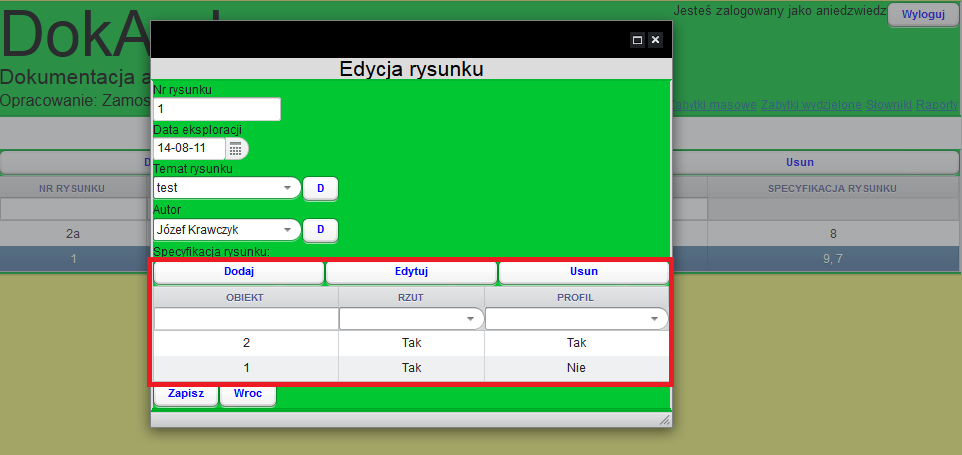
\includegraphics[scale=.6]{img/crudTable.png}
	\caption{Komponent CRUDTable (zaznaczony na czerwono)}
	\label{crudTable}
    \end{center}
\end{figure}

Nic nie stoi na przeszkodzie aby rozszerzać funkcjonalność komponentu CRUDTable. Istnieją metody, pozwalające modyfikować liste przycisków znajdujących się nad tabelą, można także dodawać pozycje widoczne w menu kontekstowym.

Dzięki wykorzystaniu komponentu FilterTable istnieje możliwość filtrowania wierszy ze względu na wartości przechowywane w konkretnych polach. Istnieje możliwość zawężenia wyświetlanych rekordów zarówno po wartościach liczbowych jak i wartościach tekstowych a nawet takich, które odwołują się do innych obiektów dziedziny problemu (czyli będących kluczem obcym).

Najważniejszą jednak funkcjonalnością jest sterowanie wyglądem treści przedstawianej przez komponent za pomocą adnotacji. Dopisując adnotacje @ColumnHeader do pola obiektu POJO definiuje się tak naprawde wygląd tabelki wyświetlającej dany obiekt. Atrybut value definiuje nam wartość widoczną w nagłówku kolumny natomiast parametr order decyduje o kolejności wyświetlanych kolumn (są one wyświetlane w kolejności rosnącej). Uwaga! To programista jest odpowiedzialny za poprawne wypełnienie wartości order, w przypadku zdublowania wartości wyświetlona zostanie tylko jedna kolumna.

Warto także dodać, że w kolumnie w sposób sensowny są takze wyświetlane inne obiekty niekoniecznie będące typami prostymi w Javie. Aby wyświetlić poprawnie obiekt, wystarczy do deklaracji klasy dodać adnotacje ForeignFieldLabel, która opisuje w jaki sposób wyświetlić wartość w danej komórce tabeli.

Obiekt, który zawiera w sobie komponent CRUDTable powinien implementować interfejs CRUDTableListener, ponieważ sam komponent nie podejmuje żadnych akcji w wyniku zdarzeń wygenerowanych przez użytkownika, a jedynie przekazuje je dalej do nasłuchiwaczy. Obiekt ten jest także odpowiedzialny za wypełnienie komponentu wartościami.
\newpage
\section{ForeignField}
Kolejnym komponentem, który wg autora może być przydatny w innych projektach jest ForeignField, który implementuje kontrolkę odpowiedzialną za wprowadzenie wartości ze słownika. Kontrolka używa komponentu ze standardowego zestawu komponentów Vaadina - ComboBox oraz przycisku.

\begin{figure} [H]
    \begin{center}
	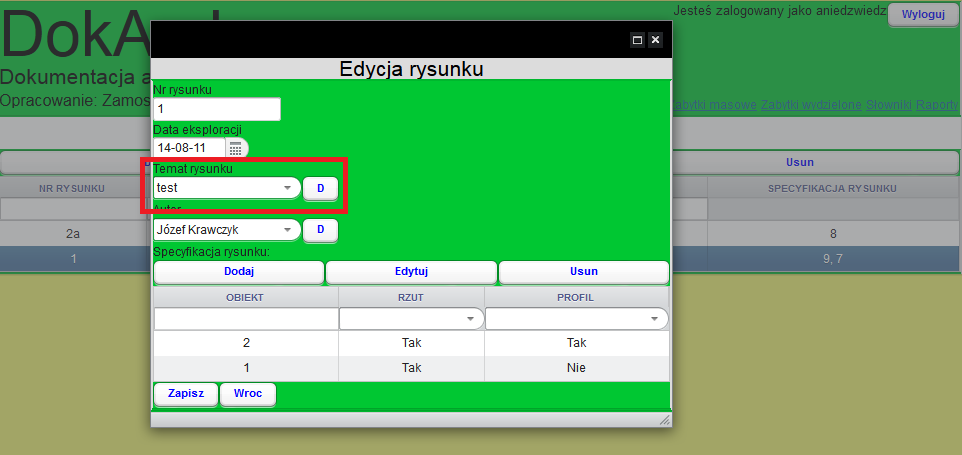
\includegraphics[scale=.6]{img/foreignField.png}
	\caption{Komponent ForeignField (zaznaczony na czerwono)}
	\label{formField}
    \end{center}
\end{figure}

Użycie kontrolki, sprowadza się do zdefiniowania wartości wyświetlanej jako wartość obiektu w liście rozwijanej (adnotacja @ForeignFieldLabel) oraz ustawienie listy możliwych wartości. Uwaga! Kontrolka sama w sobie nie podejmuje żadnych akcji po naciśnięciu przycisku. Obiekt, który zawiera w sobie komponent powinien implementować interfejs DictionaryFieldListener i tam zdefiniować zachowanie będące reakcją na naciśnięcie przycisku "D".
\section{DefaultForm}
DefaultForm jest komponentem, który na podstawie adnotacji @EditField zawartych w klasie obiektu tworzy formularz złożony z domyślnych komponentów Vaadina oraz dwóch poprzednio wymienionych: CRUDTable oraz ForeignField. 

\newpage
\begin{figure} [H]
    \begin{center}
	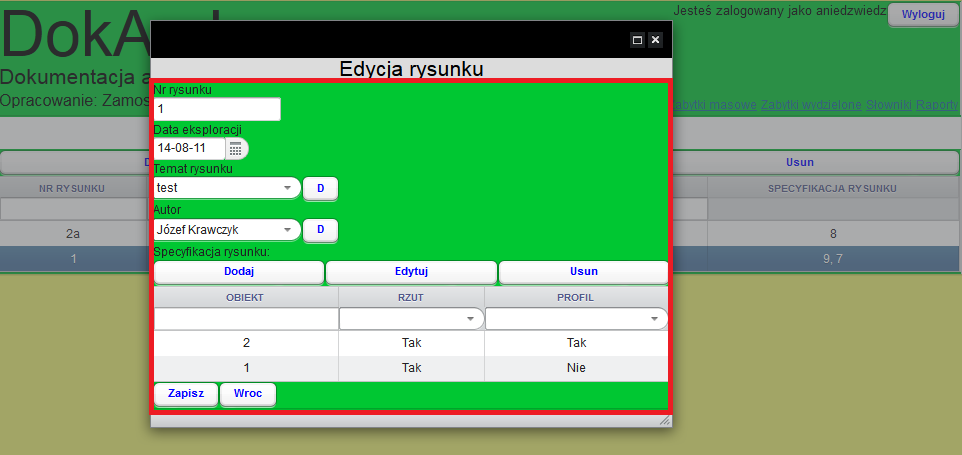
\includegraphics[scale=.6]{img/formField.png}
	\caption{Komponent FormField (zaznaczony na czerwono)}
	\label{foreignField}
    \end{center}
\end{figure}

Adnotacja @EditField zawiera w sobie informacje na temat kolejności wyświetlania komponentów do edycji kolejnych wartości obiektu (wartość order) oraz wartość etykiety (label), która powinna być wyświetlona przy danym polu. Uwaga! To programista jest odpowiedzialny za poprawne wypełnienie wartości order, w przypadku zdublowania wartości wyświetlona zostanie tylko jedno pole edycji.

Komponent DefaultForm działa deleguje zadanie tworzenia kontrolek do obiektu-fabryki implementującego interfejs ExtendedFieldGroupFieldFactory (rozszerzającego interfejs Vaadina FieldGroupFieldFactory). W zależności od typu pola obiektu tworzona jest inna kontrolka. Dla standardowych typów takich jak Integer lub String, kontrolki generowane są przez domyślną fabryke Vaadina - FieldGroupFieldFactory. W przypadku wystąpienia przy polu adnotacji javax.persistence odpowiedzialnych za relacje Wiele-Do-* lub Jeden-Do-Wielu generowana jest odpowiednia kontrolka. Jeżeli nad polem znajduje się adnotacja @ManyToOne, generowana jest kontrolka typu ForeignField, natomiast dla adnotacji @OneToMany oraz @ManyToMany, generowany jest komponent CRUDTable.

Aby wypełnić słowniki, należy dostarczyć do komponentu DefaultForm obiekt, który implementuje interfejs DataProvider, ponieważ komponent sam w sobie nie potrafi wypełnić ich wartościami.

DefaultForm nie podejmuje także samodzielnie żadnych akcji, a jedynie oddelegowuje je do zarejestrowanych listenerów. Komponent przechwytuje także zdarzenia wygenerowane w zawartych komponentach ForeignField i CRUDTable, czyli jest ich nasłuchiwaczem, jednak jedyne co robi z tymi zdarzeniami to przekazuje je dalej, dlatego istotne jest, aby obiekt zawierający w sobie komponent DefaultForm implementował interfejs FormFieldListener. Dodatkowo, aby przechwytywać zdarzenia związane z przyciskami "Zapisz" oraz "Wróć" należy zarejestrować nasłuchiwacz implementujący interfejs FormListener.

\newpage
Ważną cechą komponentu DefaultForm, o której należy wspomnieć na koniec, jest walidacja wprowadzonych wartości na podstawie adnotacji javax.validation. Wszystkie standardowe ograniczenia na wartości pól, zgodne z JSR-303 są sprawdzane przed wysłaniem akcji "zapisz" to obiektu nasłuchującego. W przypadku niepowodzenia walidacji, zdarzenie nie jest przekazywane dalej.
\section{Szkielet aplikacji przetwarzania danych biznesowych}
W trakcie tworzenia systemu wspierającego prowadzenie ewidencji badań archeologicznych powstał także szkielet aplikacji, który został opisany w rozdziale 5.

% ex: set tabstop=4 shiftwidth=4 softtabstop=4 noexpandtab fileformat=unix filetype=tex spelllang=pl,en spell:
%\chapter{Wnioski}
System wspierajacy prowadzenie dokumentacji archeologiczny, wbrew pozorom, nie jest prosty. Na szczęście współczesna informatyka dostarcza szereg narzędzi wspierających tworzenie oprogramowania dla przedsiębiorstw. 

% ex: set tabstop=4 shiftwidth=4 softtabstop=4 noexpandtab fileformat=unix filetype=tex spelllang=pl,en spell:
\chapter{Podsumowanie}
W trakcie realizacji niniejszej pracy zapoznano się z technologiami używanymi powrzechnie w przemyśle informatycznym przez firmy produkujące oprogramowanie. Dzięki użyciu najpopularniejszych technologii zapewniona była możliwość znalezienia rozwiązania problemów napotkanych w trakcie pisania pracy w internecie.

Aplikacja, która stała się produktem pracy zostanie przekazana do eksploatacji firmie "JN-Profil- badania archeologiczne i historyczne" i będzie dla niej wyraźną pomocą w generowaniu dokumentacji archeologicznej. Przyspieszy to czas jej tworzenia, co wpłynie na zmniejszenie kosztów jej tworzenia. 

Pomimo tego, że dziedzina problemu raczej nie powinna ulegać zmianie, to istnieje prawdopodobieństwo, że dokumentacja archeologiczna może wymagać dokumentów, których wygenerowanie nie zostało zapewnione przez system stworzony w ramach niniejszej pracy inżynierskiej. Jeżeli zajdzie potrzeba, system jest w łatwy sposób rozszerzalny i jego rozwój jest jak najbardziej planowany w przyszłości.

Dodatkowymi produktami powstałymi w trakcie pisania niniejszej pracy powstały komponenty CRUDTable, ForeignField, DefaultForm oraz szkielet aplikacji użyty do tworzenia pracy. Wszystkie komponenty w niedługiej przyszłości zostaną zgłoszone do twórców szkieletu aplikacji jako kandydat na wtyczke ułatwiającą prace programistom, którzy wyrali pracę z Vaadinem.
% ex: set tabstop=4 shiftwidth=4 softtabstop=4 noexpandtab fileformat=unix filetype=tex spelllang=pl,en spell:

\appendix

% tutaj załączniki

%\chapter*{Bibliografia}
\nocite{*}
\bibliographystyle{plplain}
%\bibliographystylebk{plplain}
%\bibliographystylest{plplain}
%\bibliographystyledoc{plplain}
% \bibliographystyleweb{plplain}
%\bibliographybk{BIB/books}
%\bibliographyst{BIB/books}
%\bibliographydoc{BIB/books}
% \bibliographyweb{BIB/books}

% \bibliography{bib/verificard,bib/jml,bib/daikon}
%\bibliography{bib/daikon,bib/statistics,bib/other}
\bibliography{bib/other}

\end{document}

% ex: set tabstop=4 shiftwidth=4 softtabstop=4 noexpandtab fileformat=unix filetype=tex spelllang=pl,en spell:

